\section{结果}

\subsection{原始临床基线模型}
在直接使用原始术前临床变量的患者级 Logistic 回归分析中，CentralLNM 的平均测试 AUC 为 0.6859$\pm$0.0658，ACC、F1、Sen 和 Spe 分别为 0.6332、0.6661、0.6712 和 0.5881，说明即使不引入深度影像特征，临床变量本身已具备较强判别力。

\begin{table}[H]
\centering
\caption{原始术前临床变量构建的 CentralLNM 基线结果（患者级 5-fold）}
\label{tab:raw_clinical_central}
\begin{tabular}{lccccc}
\toprule
任务 & AUC Mean$\pm$Std & ACC & F1 & Sen & Spe \\
\midrule
CentralLNM & $0.6859\pm0.0658$ & 0.6332 & 0.6661 & 0.6712 & 0.5881 \\
\bottomrule
\end{tabular}
\end{table}

\begin{table}[H]
\centering
\caption{CentralLNM 原始临床基线中跨折最稳定的关键特征}
\label{tab:clinical_predictors_central}
\small
\begin{tabular}{p{0.34\textwidth}ccc}
\toprule
特征 & 单因素显著频次 & 多因素入选频次 & 多因素中位 OR \\
\midrule
年龄（每增 1 岁） & 5/5 & 5/5 & $\approx 0.96$ \\
微钙化 & 5/5 & 5/5 & $\approx 2.09$ \\
超声提示中央区淋巴结异常 & 4/5 & 5/5 & $\approx 4.03$ \\
性别（男） & 4/5 & 4/5 & $\approx 1.67$ \\
病灶长径 & 4/5 & 4/5 & $\approx 2.74$ \\
病灶前后径 & 4/5 & 4/5 & $\approx 2.12$ \\
\bottomrule
\end{tabular}
\end{table}


\begin{figure}[H]
\centering
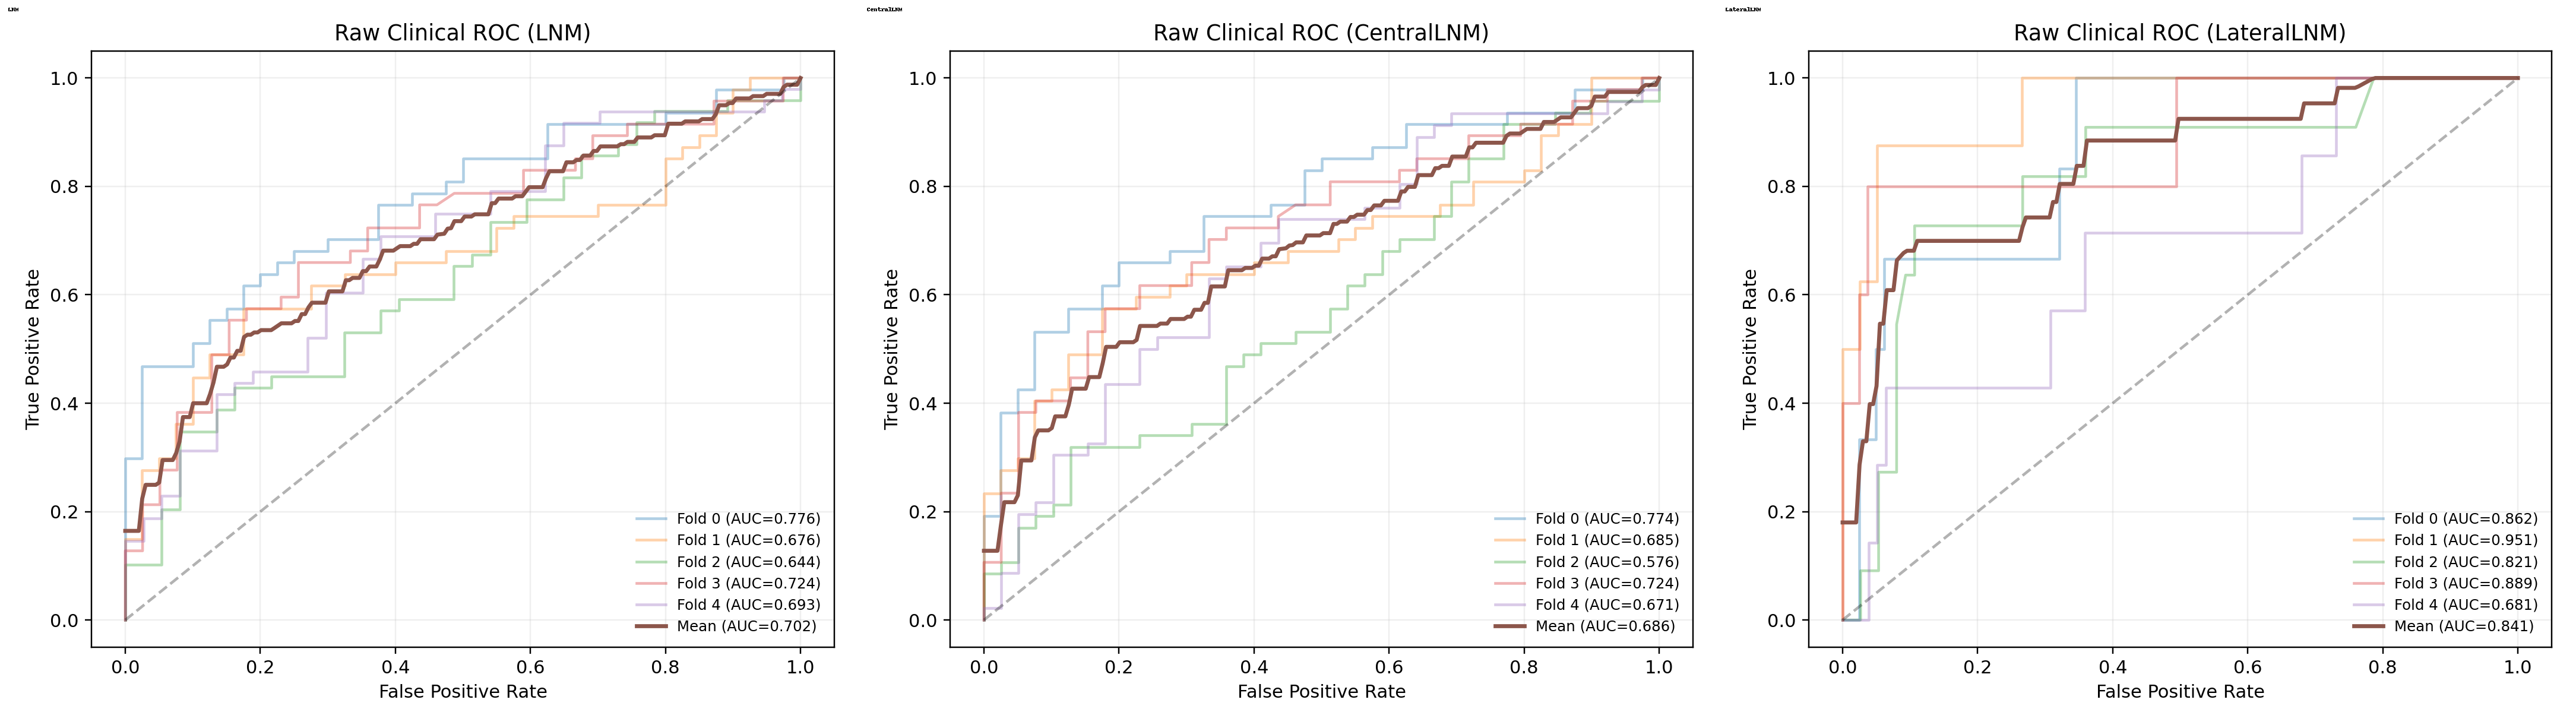
\includegraphics[width=0.92\textwidth]{figures/raw_clinical_roc_panel.png}
\caption{原始临床回归基线在 LNM、CentralLNM 与 LateralLNM 三任务中的 ROC 曲线。本文主终点为 CentralLNM，其余任务用于提供背景性参照。}
\label{fig:raw_clinical_roc}
\end{figure}

从变量稳定性来看，年龄、微钙化、术前超声提示中央区淋巴结异常以及病灶尺寸是跨折最稳定的 CentralLNM 相关因素。该结果提示，在当前数据条件下，最可复核且最具临床解释性的风险信号仍主要来自术前临床与常规超声描述。由此，原始临床回归应作为全文的核心参照基线，而非边缘对照。
图~\ref{fig:raw_clinical_roc} 显示，原始临床模型在 CentralLNM 任务上呈现连续且平滑的 ROC 形态，说明其风险排序能力并非由个别阈值点驱动。与此同时，LateralLNM 虽出现较高曲线下面积，但其阈值相关指标并不理想，进一步支持“非主终点结果仅作补充说明”的写作策略。

\subsection{ROI radiomics 方法}
在统一患者级 5-fold 协议下，3.2 节替换为 ROI radiomics 两条 pipeline：ROI Radiomics-only 与 Clinical+ROI Radiomics。结果显示，ROI Radiomics-only 的判别能力有限，而 Clinical+ROI Radiomics 在多模型下均表现出更稳定的提升趋势。

\begin{table}[H]
\centering
\caption{ROI radiomics 两条路径的最佳结果汇总（患者级 5-fold）}
\label{tab:traditional_radiomics}
\small
\begin{tabular}{lcccccc}
\toprule
路径 & 最佳模型 & AUC Mean$\pm$Std & ACC & F1 & Sen & Spe \\
\midrule
ROI Radiomics-only & LogReg & $0.5756\pm0.0538$ & 0.5566 & 0.6151 & 0.6536 & 0.4417 \\
Clinical+ROI Radiomics & SoftVoting & $0.6923\pm0.0696$ & 0.6330 & 0.6672 & 0.6839 & 0.5729 \\
\bottomrule
\end{tabular}
\end{table}

\begin{table}[H]
\centering
\caption{ROI radiomics 多模型比较（仅保留两条 pipeline，按 AUC 均值降序）}
\label{tab:traditional_multimodel}
\small
\begin{tabular}{llc}
\toprule
Pipeline & 模型 & AUC Mean$\pm$Std \\
\midrule
Clinical+ROI Radiomics & SoftVoting & $0.6923\pm0.0696$ \\
Clinical+ROI Radiomics & RandomForest & $0.6901\pm0.0486$ \\
Clinical+ROI Radiomics & Stacking & $0.6864\pm0.0741$ \\
Clinical+ROI Radiomics & LogReg & $0.6848\pm0.0785$ \\
Clinical+ROI Radiomics & ExtraTrees & $0.6775\pm0.0628$ \\
Clinical+ROI Radiomics & SVM(RBF) & $0.6745\pm0.0448$ \\
Clinical+ROI Radiomics & AdaBoost & $0.5846\pm0.0428$ \\
\midrule
ROI Radiomics-only & LogReg & $0.5756\pm0.0538$ \\
ROI Radiomics-only & Stacking & $0.5735\pm0.0520$ \\
ROI Radiomics-only & SVM(RBF) & $0.5735\pm0.0422$ \\
ROI Radiomics-only & SoftVoting & $0.5665\pm0.0550$ \\
ROI Radiomics-only & RandomForest & $0.5521\pm0.0458$ \\
ROI Radiomics-only & ExtraTrees & $0.5359\pm0.0616$ \\
ROI Radiomics-only & AdaBoost & $0.5298\pm0.0547$ \\
\bottomrule
\end{tabular}
\end{table}


具体而言，ROI Radiomics-only 的最佳 AUC 为 0.5756$\pm$0.0538；Clinical+ROI Radiomics 的最佳 AUC 为 0.6923$\pm$0.0696，在多模型比较中持续优于 ROI Radiomics-only。该结果进一步支持“仅依赖组学特征不足以满足临床判别需求”，而临床信息与 ROI radiomics 的联合建模具有更高应用价值。

\subsection{多模态深度学习融合}
在多模态深度学习部分，本文将 Ours 方法统一替换为性能最高的 ViT-B/16 对应结果，并与临床基线及传统影像组学在同一比较框架下展示。

\begin{table}[H]
\centering
\caption{CentralLNM 主文核心路径的统一比较}
\label{tab:main_route_comparison}
\footnotesize
\setlength{\tabcolsep}{4pt}
\begin{tabular}{lccccccc}
\toprule
方法 & AUC Mean$\pm$Std & ACC & F1 & Sen & Spe & Compliance \\
\midrule
原始临床 Logistic（Baseline） & $0.6859\pm0.0658$ & 0.6332 & 0.6661 & 0.6712 & 0.5881 & -- \\
ROI Radiomics-only & $0.5756\pm0.0538$ & 0.5566 & 0.6151 & 0.6536 & 0.4417 & -- \\
Clinical+ROI Radiomics & $0.6923\pm0.0696$ & 0.6330 & 0.6672 & 0.6839 & 0.5729 & -- \\
Ours（ViT-B/16） & $\mathbf{0.7104\pm0.0253}$ & 0.6289 & 0.6686 & 0.6969 & 0.5490 & $0.9512\pm0.0626$ \\
\bottomrule
\end{tabular}
\end{table}

\begin{table}[H]
\centering
\caption{相对原始临床基线的增量价值总结（CentralLNM，患者级 5-fold）}
\label{tab:incremental_value}
\small
\begin{tabular}{lccc}
\toprule
路径 & AUC$\pm$Std & $\Delta$AUC vs Baseline & 波动变化 \\
\midrule
原始临床 Logistic & $0.6859\pm0.0658$ & 参考 & 参考 \\
ROI Radiomics-only & $0.5756\pm0.0538$ & $-0.1103$ & 略下降 \\
Clinical+ROI Radiomics & $0.6923\pm0.0696$ & $+0.0064$ & 略上升 \\
Deep+Clinical（ViT-B/16） & $\mathbf{0.7104\pm0.0253}$ & $\mathbf{+0.0245}$ & 明显下降 \\
Tri-Fusion（ViT-B/16） & $0.6404\pm0.0496$ & $-0.0455$ & 下降 \\
\bottomrule
\end{tabular}
\end{table}


从统一对照可见，ViT-B/16 对应的 Ours 模型在 CentralLNM 上达到 0.7104$\pm$0.0253 的 AUC，为当前主文中最高的深度学习结果。相对于原始临床基线，其绝对增益为 0.0245，且折间标准差由 0.0658 降至 0.0253；相比之下，Clinical+ROI Radiomics 虽略高于原始临床（$\Delta$AUC=0.0064），但稳定性未见同步改善。该结果提示，在保持相同融合框架的前提下，骨干表征能力与融合方式共同决定了影像信息能否形成真正有意义的临床增量。

\begin{figure}[H]
\centering
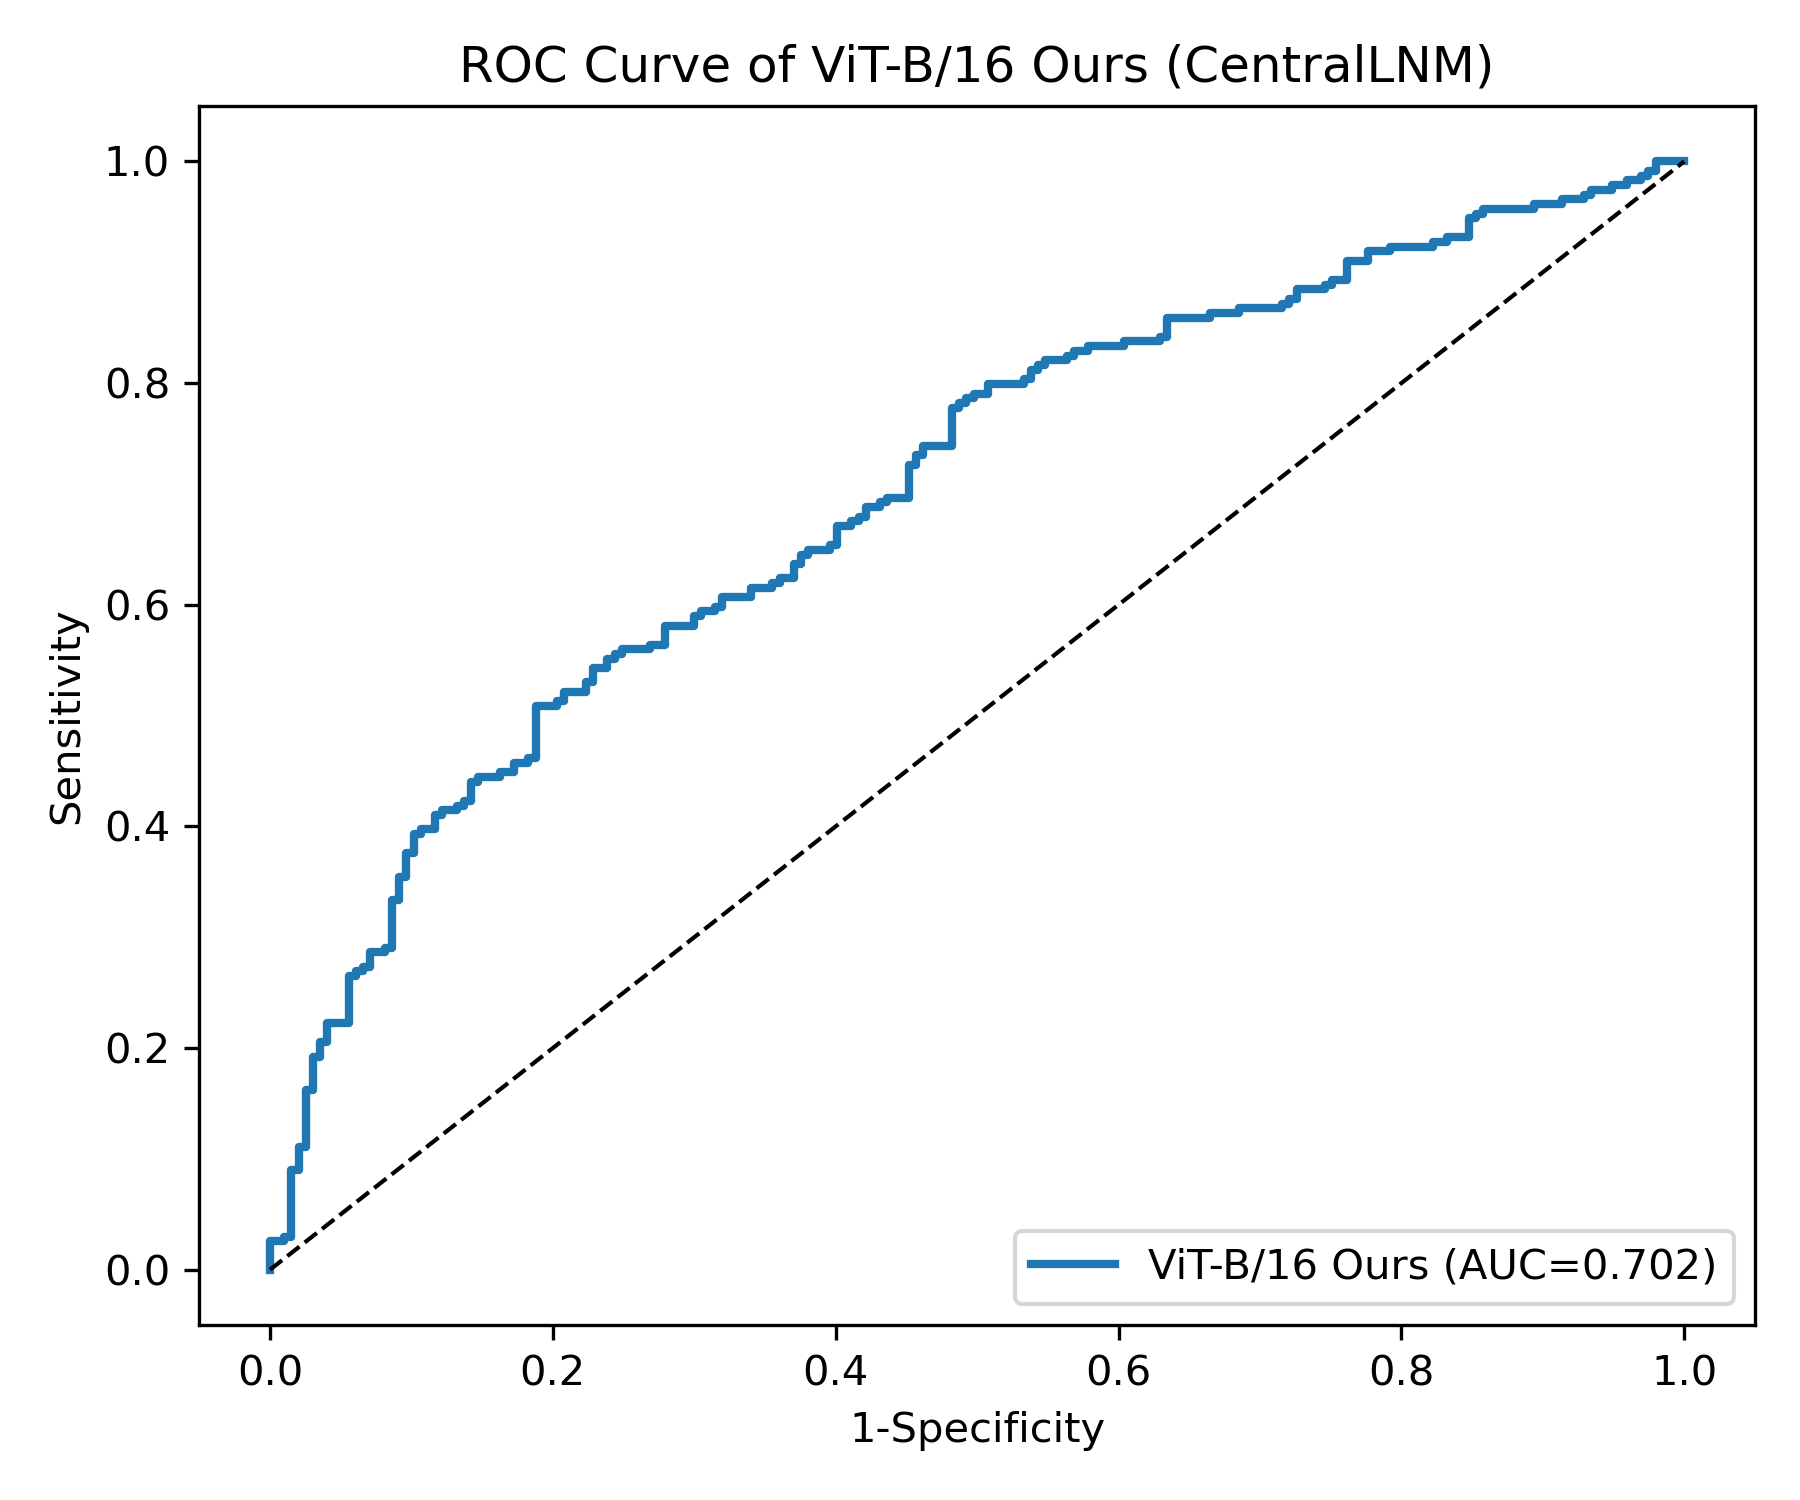
\includegraphics[width=0.78\textwidth]{figures/roc_overlay_ours_vit_b16.png}
\caption{ViT-B/16 对应 Ours 模型在 CentralLNM 任务上的患者级 5-fold ROC 叠加曲线。}
\label{fig:ours_roc}
\end{figure}

\begin{figure}[H]
\centering
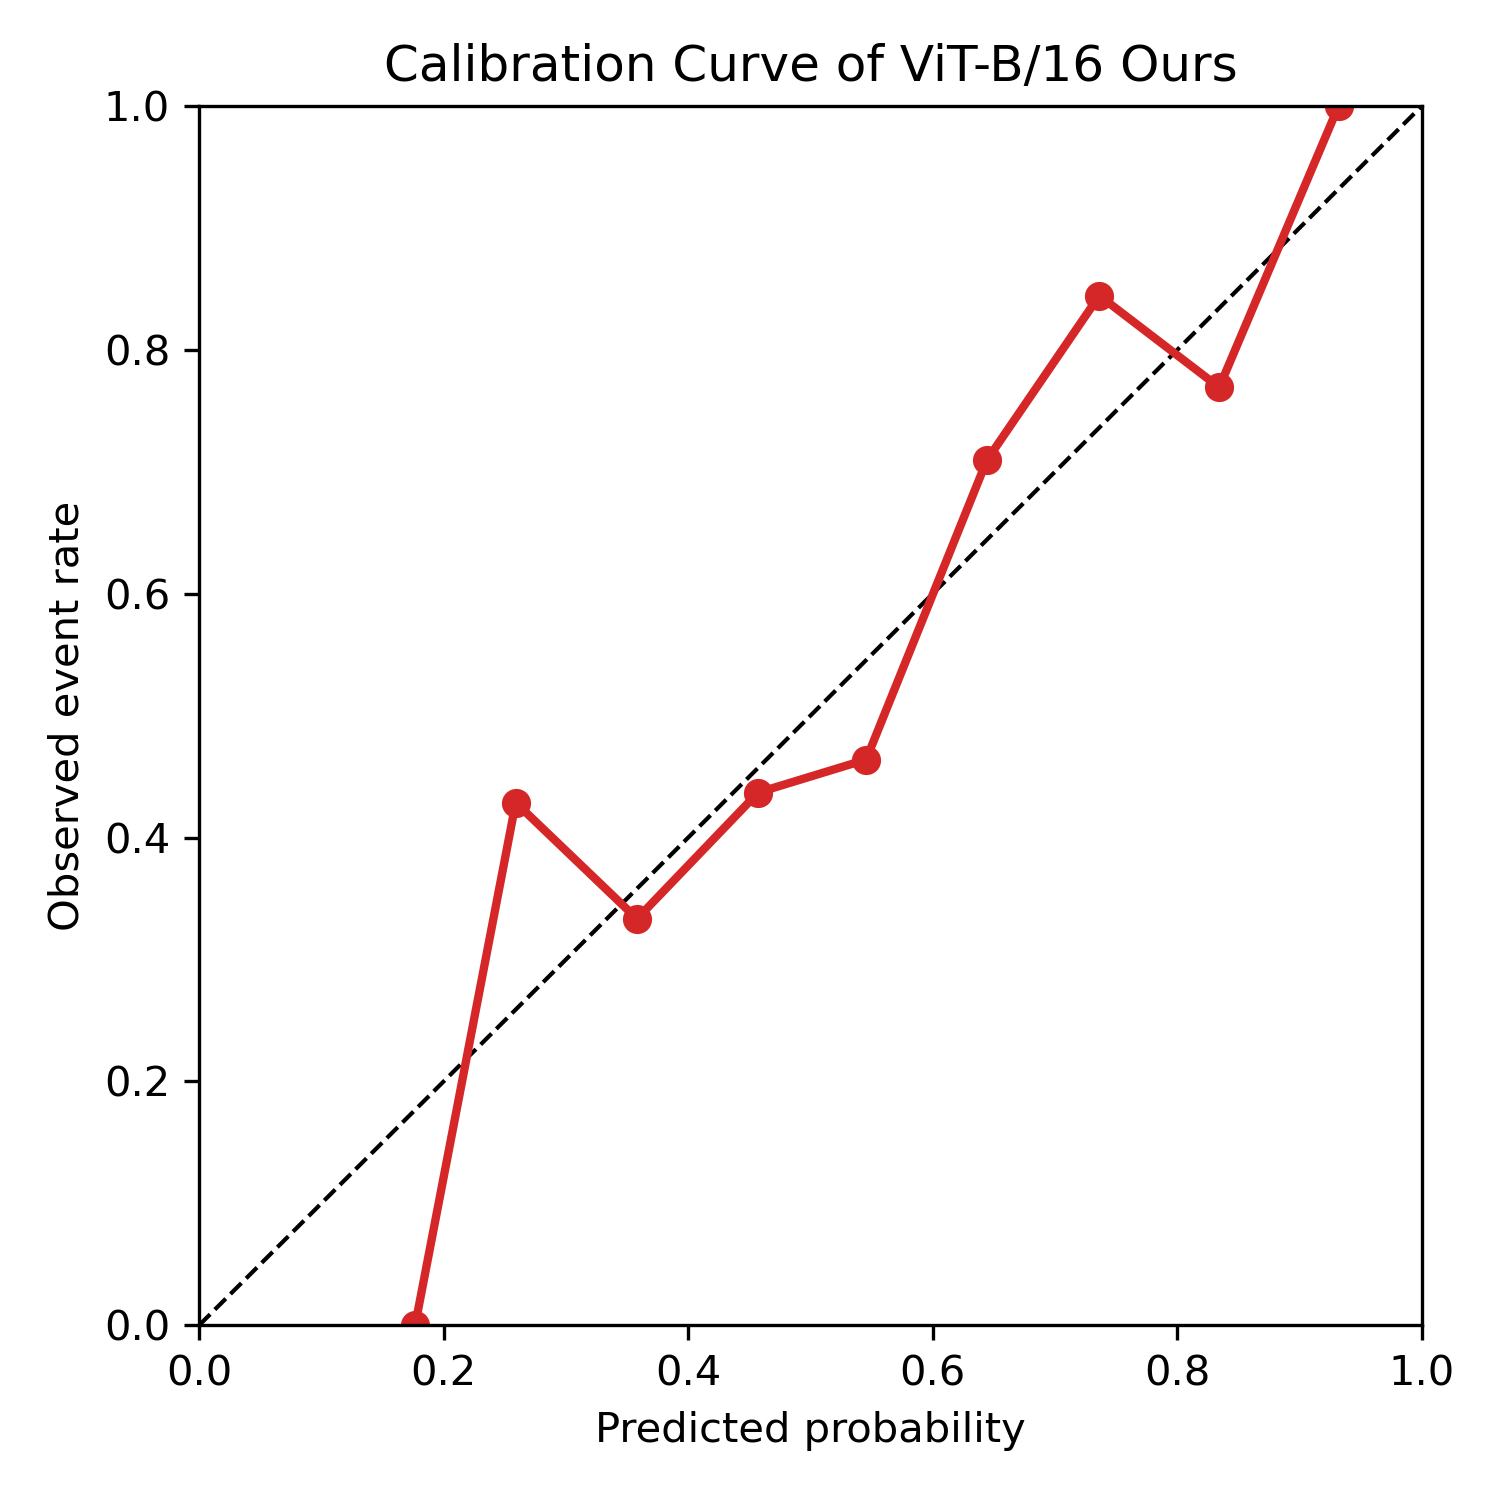
\includegraphics[width=0.55\textwidth]{figures/calibration_ours_vit_b16.png}
\caption{ViT-B/16 对应 Ours 模型在 CentralLNM 任务上的校准曲线。}
\label{fig:ours_calibration}
\end{figure}

\begin{figure}[H]
\centering
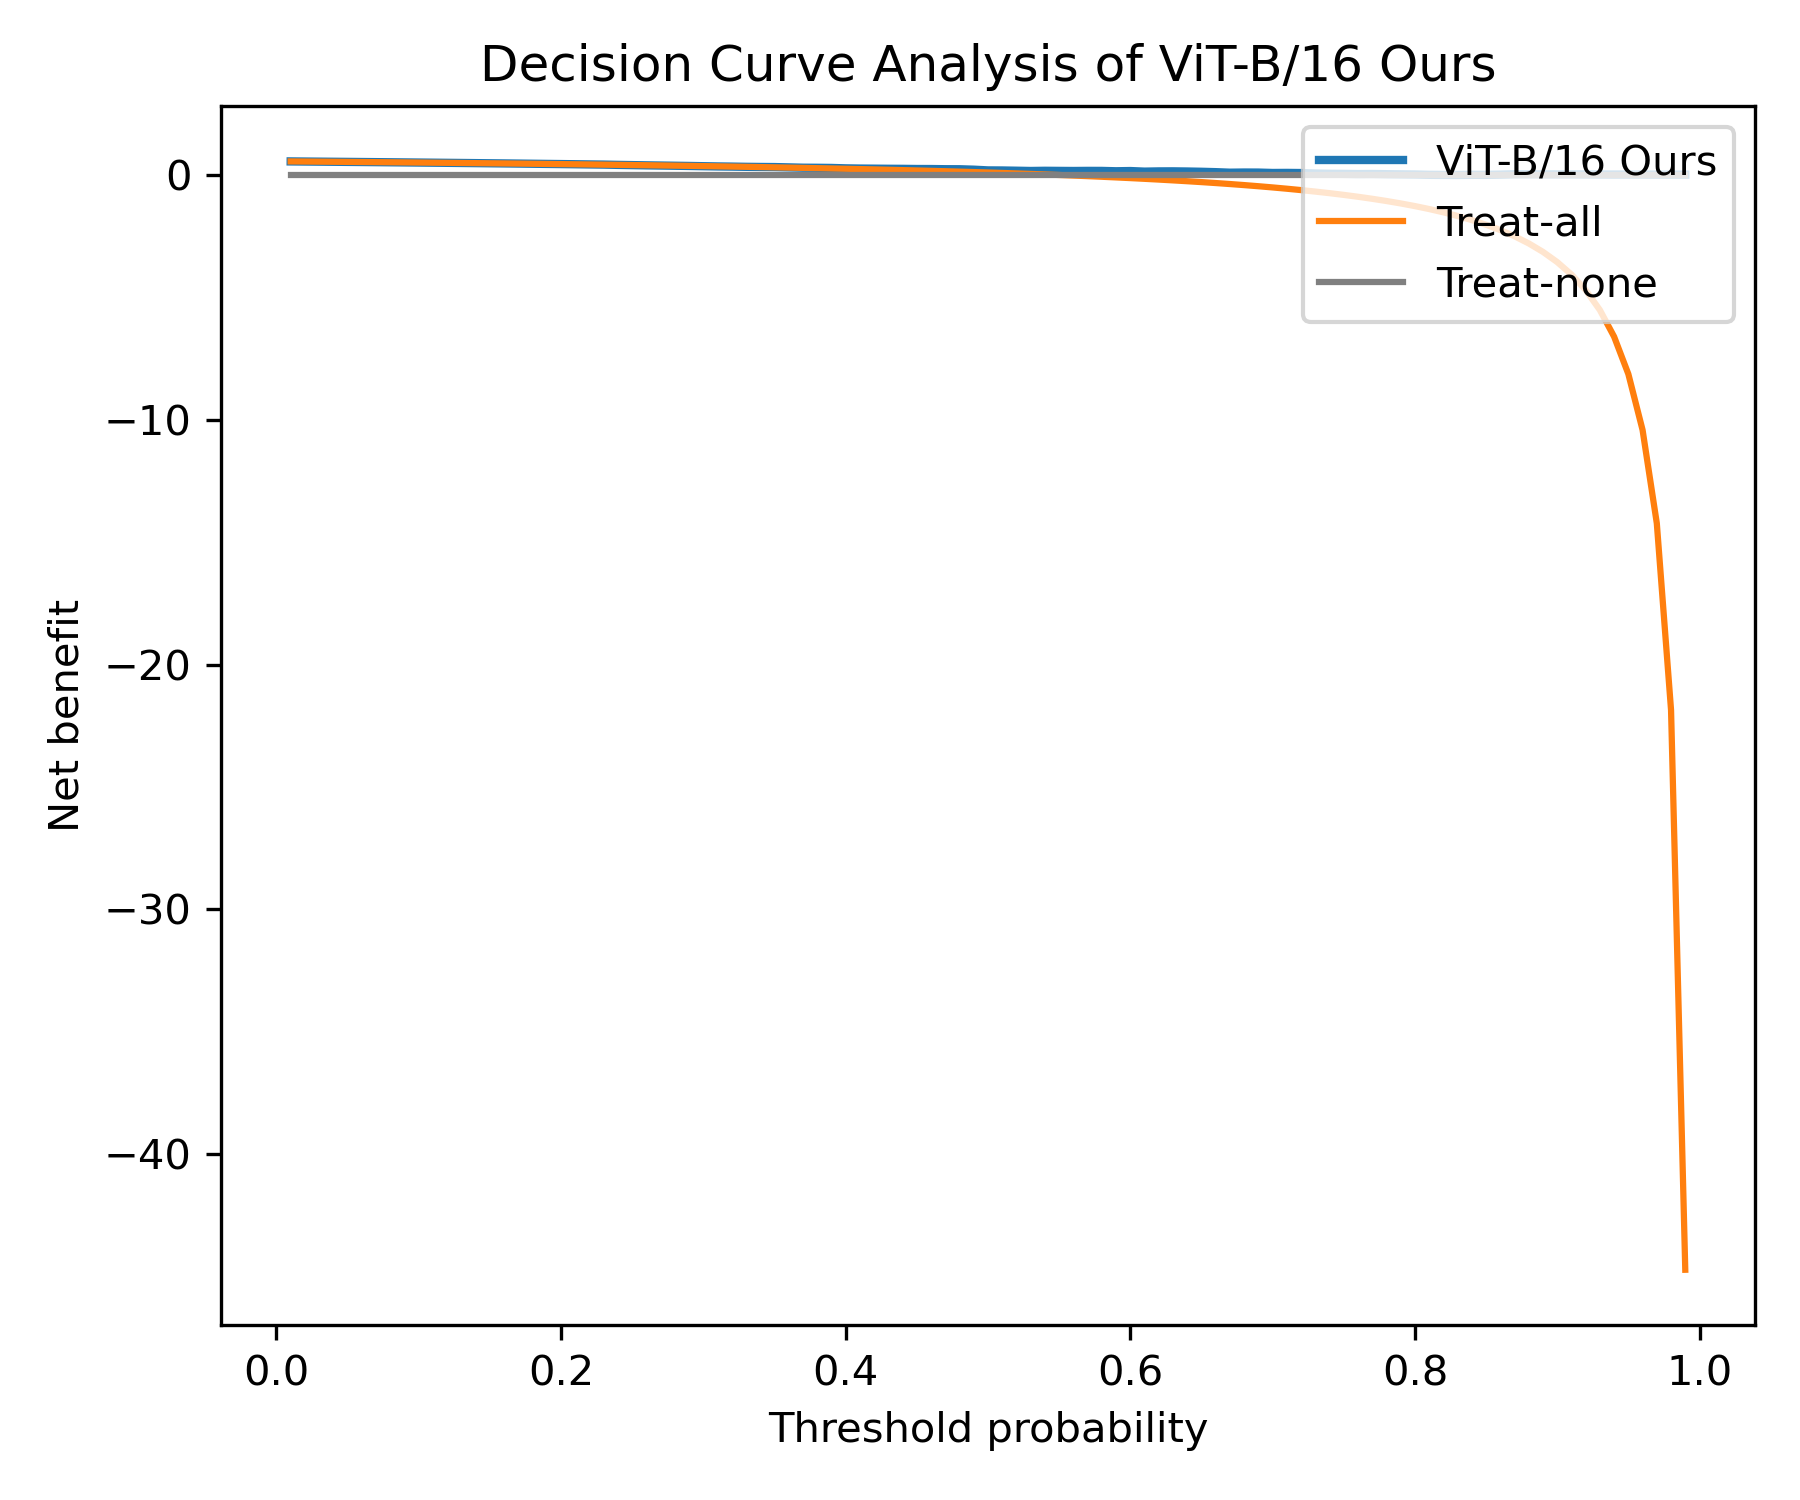
\includegraphics[width=0.68\textwidth]{figures/dca_ours_vit_b16.png}
\caption{ViT-B/16 对应 Ours 模型在 CentralLNM 任务上的决策曲线分析（decision curve analysis, DCA）。}
\label{fig:ours_dca}
\end{figure}

图~\ref{fig:ours_roc} 显示，ViT-B/16 对应模型在 5 折测试中保持稳定的 ROC 表现。图~\ref{fig:ours_calibration} 表明其预测概率与观测事件率总体一致。图~\ref{fig:ours_dca} 进一步提示，该模型在临床阈值范围内具有良好的净获益趋势。结合表~\ref{tab:incremental_value} 可见，当前最有价值的结论并非“影像全面替代临床”，而是“在原始临床基线已经较强的前提下，结构化深度融合仍可提供有限但更稳定的增量信息”。

\subsection{多架构公平比较与消融验证}
在统一预训练协议下，不同骨干网络的表现存在明显权衡关系。ViT-B/16 获得最高的 CentralLNM AUC（0.7104$\pm$0.0253），MobileViT-S 的灵敏度最高，而 Swin-T 在特异度与依从率方面更为突出。

\begin{table}[H]
\centering
\caption{统一预训练协议下 8 种骨干网络的患者级 5-fold 汇总比较}
\label{tab:backbone_compare}
\small
\begin{tabular}{lcccccc}
\toprule
Backbone & Central AUC & ACC & F1 & Sen & Spe & Compliance \\
\midrule
ViT-B/16 & $\mathbf{0.7104\pm0.0253}$ & 0.6289 & 0.6686 & 0.6969 & 0.5490 & $0.9512\pm0.0626$ \\
MobileViT-S & $0.6995\pm0.0463$ & 0.6244 & 0.6817 & 0.7521 & 0.4740 & $0.9746\pm0.0268$ \\
ResNet18 & $0.6963\pm0.0115$ & 0.6244 & 0.6745 & 0.7178 & 0.5137 & $0.9768\pm0.0317$ \\
Swin-T & $0.6939\pm0.0267$ & 0.6473 & 0.6620 & 0.6635 & 0.6296 & $\mathbf{0.9977\pm0.0047}$ \\
EffNet-B2 & $0.6861\pm0.0268$ & 0.6170 & 0.6613 & 0.7148 & 0.5022 & $0.9744\pm0.0173$ \\
EffNet-B0 & $0.6732\pm0.0236$ & 0.6173 & 0.6592 & 0.7014 & 0.5178 & $0.9700\pm0.0382$ \\
ConvNeXt-T & $0.6645\pm0.0267$ & 0.6379 & 0.6762 & 0.7179 & 0.5432 & $0.9883\pm0.0148$ \\
ResNet50 & $0.6514\pm0.0223$ & 0.5687 & 0.6206 & 0.6759 & 0.4423 & $0.9791\pm0.0226$ \\
\bottomrule
\end{tabular}
\end{table}


\begin{figure}[H]
\centering
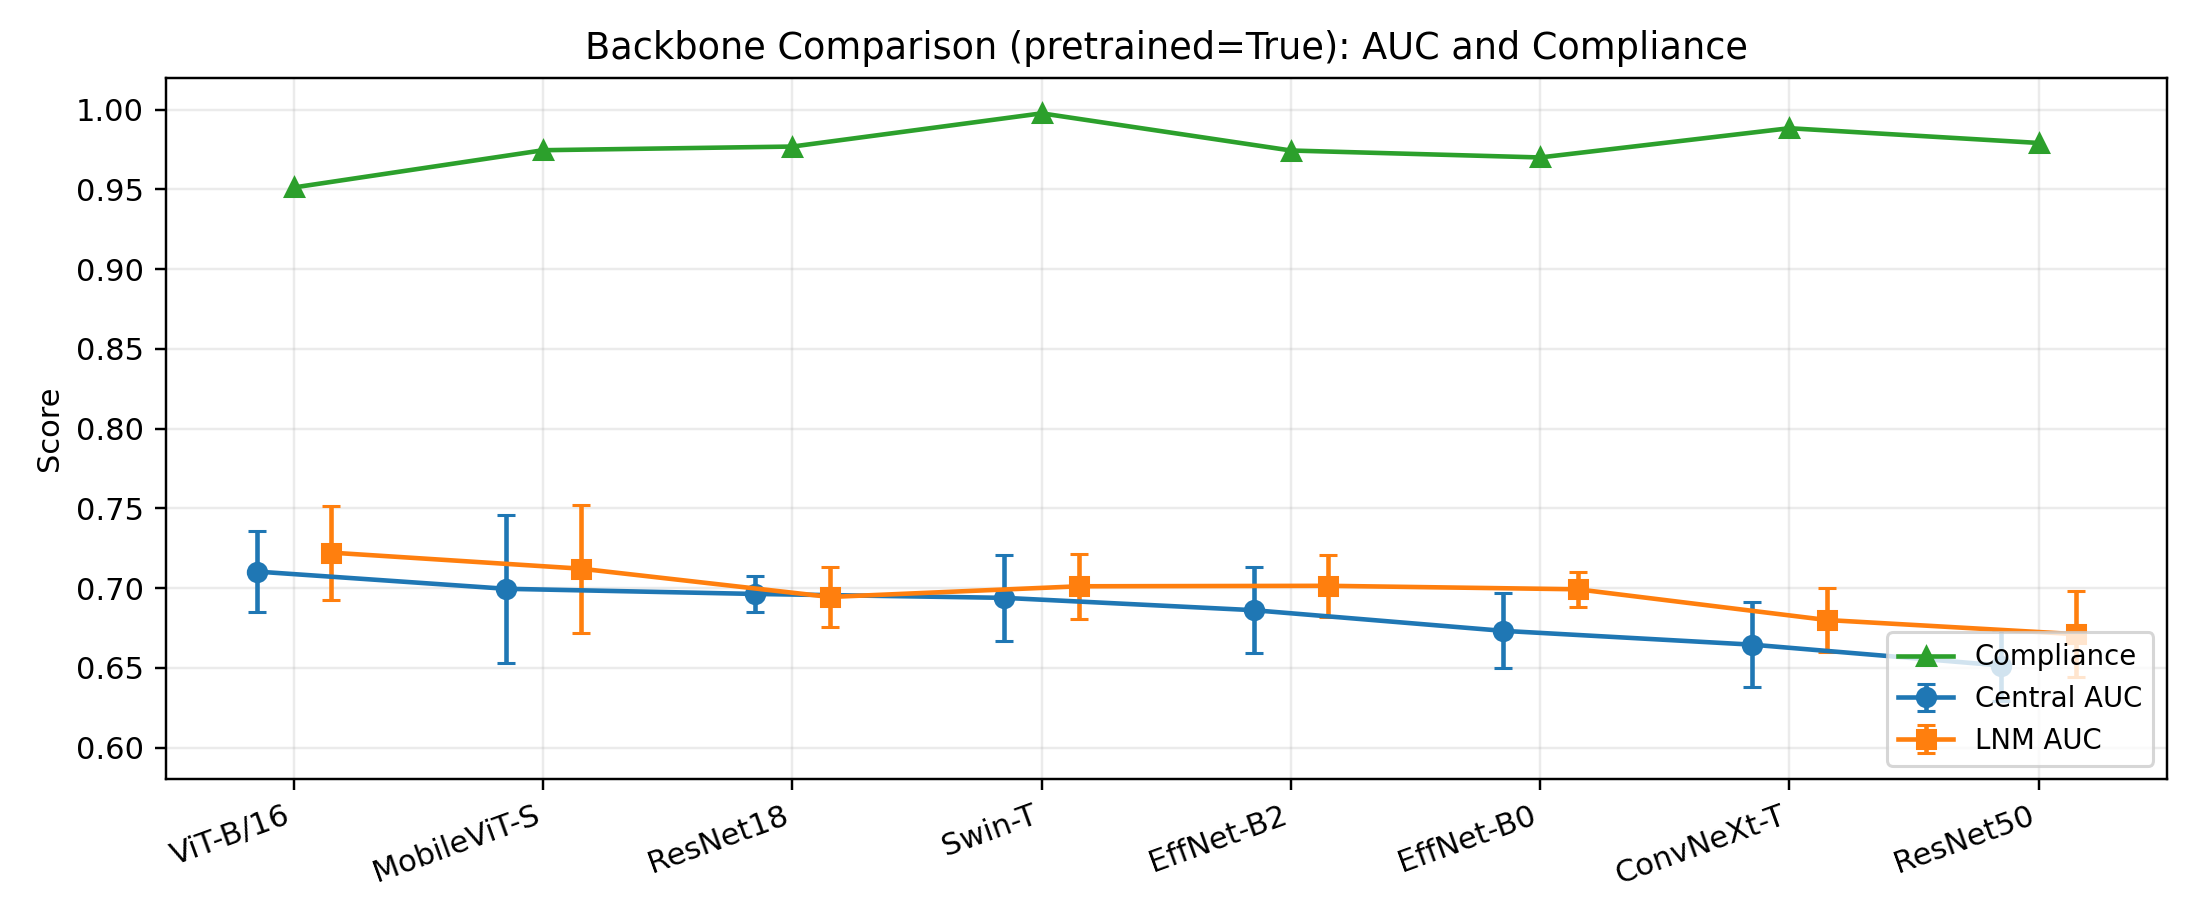
\includegraphics[width=0.88\textwidth]{figures/backbone_auc_compliance.png}
\caption{不同骨干网络在 CentralLNM AUC 与逻辑依从率上的比较。误差线表示 5-fold 标准差。}
\label{fig:backbone_compare}
\end{figure}

结果表明，当前任务不存在在全部指标上同时占优的单一骨干；若强调排序能力，ViT-B/16 更具优势；若强调规则一致性与误报控制，Swin-T 更具参考价值。因此，多架构比较在本文中定位为“稳健性分析”，而非主文核心终点结论。
图~\ref{fig:backbone_compare} 直观呈现了该权衡关系：ViT-B/16 的 AUC 最高，但依从率并非最优；Swin-T 在 AUC 略低条件下保持了更稳定的一致性表现。该结果提示，骨干选择应围绕临床目标进行多指标联合决策，而非仅依据单一 AUC 排序。

相比之下，关键模块消融更直接回答“为什么完整模型成立”。在剔除 Base-A（Clinical-only）后，消融结果仍显示 Ours 方案在 AUC 上保持最高水平，说明患者级 MIL、门控融合与先验约束的组合具有稳定增益。

\begin{table}[H]
\centering
\caption{五组消融的全指标对照（CentralLNM，患者级 5-fold）}
\label{tab:ablation_full_metrics}
\footnotesize
\setlength{\tabcolsep}{4pt}
\begin{tabular}{lcccccc}
\toprule
设置 & AUC & ACC & F1 & Sen & Spe & Compliance \\
\midrule
Base-B（SliceMean+Concat） & $0.6724\pm0.0326$ & 0.6291 & 0.6881 & 0.7567 & 0.4786 & $0.4464\pm0.2409$ \\
Abl-1（MeanMIL+Gated） & $0.6891\pm0.0419$ & 0.6266 & 0.6213 & 0.6034 & 0.6562 & $0.9883\pm0.0105$ \\
Abl-2（AttMIL+Concat） & $0.6672\pm0.0360$ & 0.5988 & 0.6081 & 0.5989 & 0.6001 & $0.9930\pm0.0093$ \\
Abl-3（NoPrior） & $0.6632\pm0.0235$ & 0.6035 & 0.6152 & 0.6035 & 0.6040 & $0.6518\pm0.0476$ \\
Ours（ViT-B/16） & $\mathbf{0.7104\pm0.0253}$ & 0.6289 & 0.6686 & 0.6969 & 0.5490 & $0.9512\pm0.0626$ \\
\bottomrule
\end{tabular}
\end{table}

\begin{table}[H]
\centering
\caption{ViT-B/16 完整模型的 CentralLNM 风险分层表现}
\label{tab:calib_strata}
\small
\begin{tabular}{p{0.24\textwidth}ccc}
\toprule
风险分层（$\hat{p}_{central}$） & $N$ & 阳性例数 & 观察阳性率 \\ 
\midrule
0.1$\sim$0.2 & 2 & 0 & 0.000 \\ 
0.2$\sim$0.3 & 14 & 6 & 0.429 \\ 
0.3$\sim$0.4 & 60 & 20 & 0.333 \\ 
0.4$\sim$0.5 & 103 & 45 & 0.437 \\ 
0.5$\sim$0.6 & 97 & 45 & 0.464 \\ 
0.6$\sim$0.7 & 93 & 66 & 0.710 \\ 
0.7$\sim$0.8 & 45 & 38 & 0.844 \\ 
0.8$\sim$0.9 & 13 & 10 & 0.769 \\ 
0.9$\sim$1.0 & 4 & 4 & 1.000 \\ 
\bottomrule
\end{tabular}
\end{table}


\begin{figure}[H]
\centering
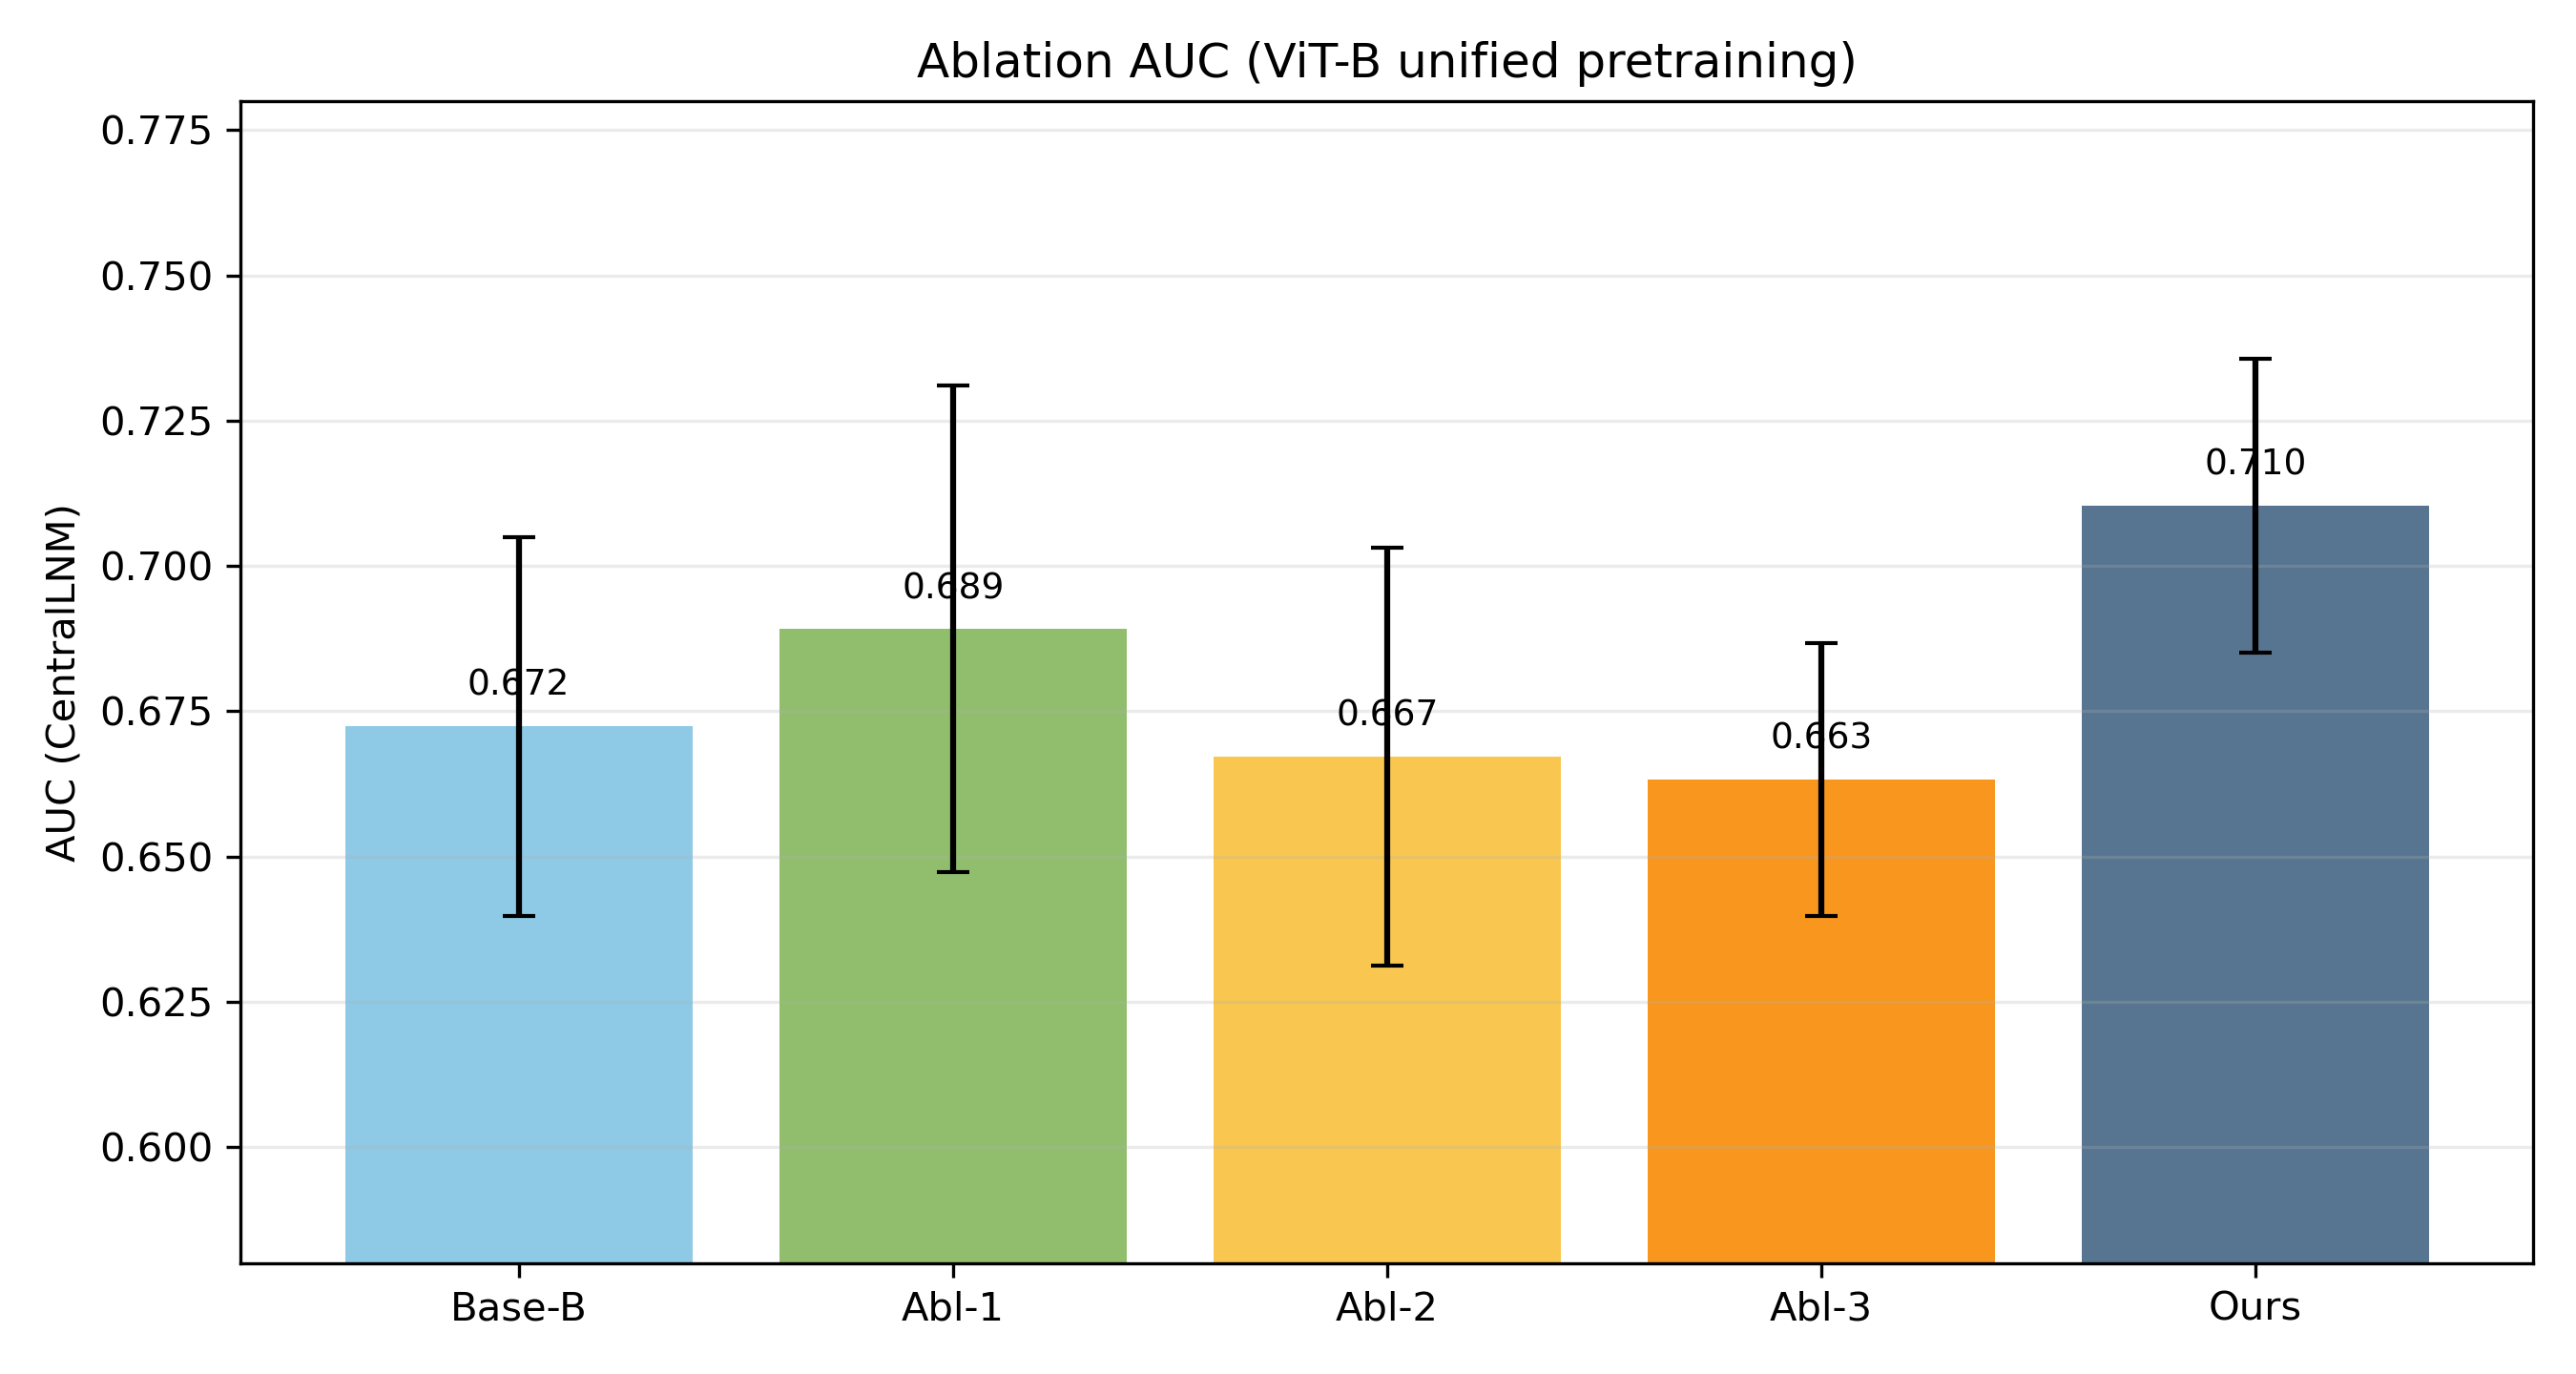
\includegraphics[width=0.86\textwidth]{figures/auc_bar_v2_ablation5_vit.png}
\caption{剔除 Base-A 后的五组消融在 CentralLNM 任务上的 AUC 比较（Ours 为 ViT-B/16 结果）。}
\label{fig:ablation_auc}
\end{figure}

\begin{figure}[H]
\centering
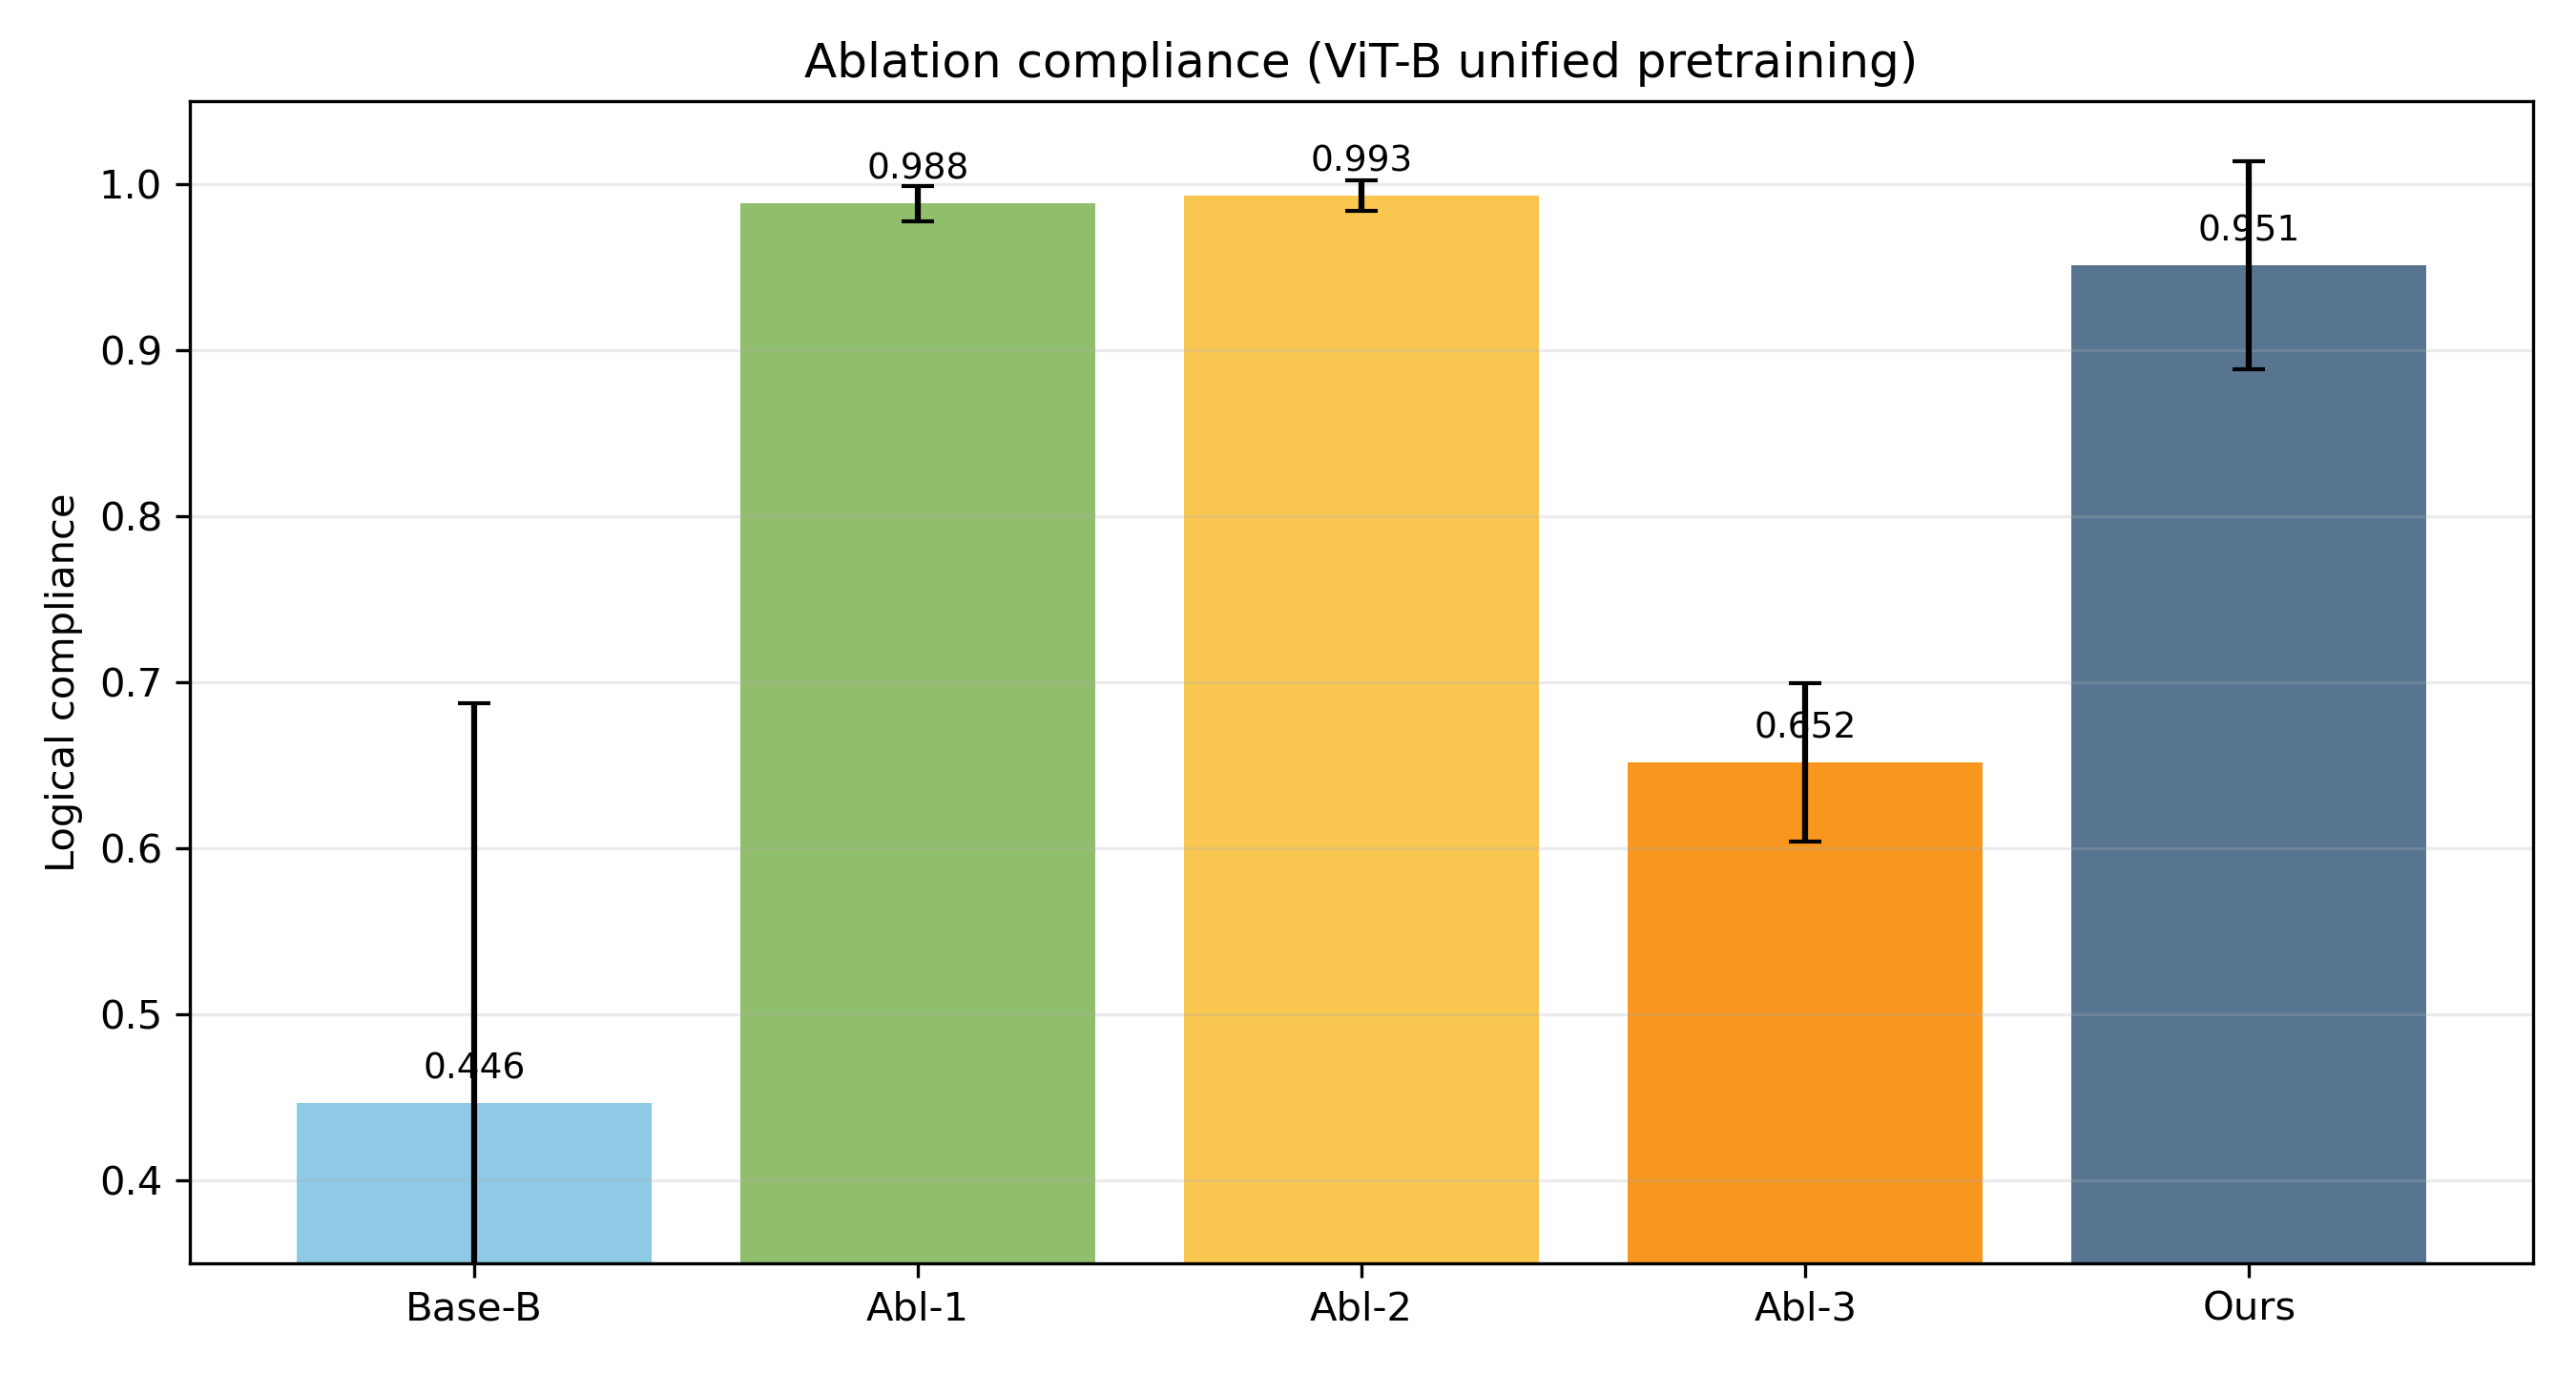
\includegraphics[width=0.86\textwidth]{figures/compliance_bar_v2_ablation5_vit.png}
\caption{剔除 Base-A 后的五组消融在逻辑依从率上的比较（Ours 为 ViT-B/16 结果）。}
\label{fig:ablation_compliance}
\end{figure}

具体而言，Mean-MIL + Gated 的结果仍优于 Attention-MIL + Concat，提示临床主导门控优于直接拼接。去除先验约束后，依从率出现显著下降，说明先验项在维持临床逻辑一致性方面仍是关键模块。风险分层表亦显示，随着预测风险升高，真实阳性率总体上升，支持模型输出的分层解释价值。
图~\ref{fig:ablation_auc} 与图~\ref{fig:ablation_compliance} 为上述结论提供了直观证据：在剔除临床-only 基线后，Ours（ViT-B/16）仍保持最高 AUC，并维持较高逻辑一致性，提示该框架具有较好的临床可迁移性。

\subsection{多源融合验证}
在深度学习与临床融合基础上引入 ROI radiomics 分支后，本节统一替换为 ViT-B/16 对应结果，比较 ROI Radiomics-only、Clinical+ROI Radiomics、V1（Deep+Clinical）与 V2（Tri-Fusion）。

\begin{table}[H]
\centering
\caption{多源融合验证结果汇总（CentralLNM，患者级 5-fold）}
\label{tab:tri_source}
\footnotesize
\setlength{\tabcolsep}{4pt}
\begin{tabular}{lcccccc}
\toprule
设置 & AUC$\pm$Std & ACC & F1 & Sen & Spe & Compliance \\
\midrule
ROI Radiomics-only & $0.5756\pm0.0538$ & 0.5566 & 0.6151 & 0.6536 & 0.4417 & -- \\
Clinical+ROI Radiomics & $0.6923\pm0.0696$ & 0.6330 & 0.6672 & 0.6839 & \textbf{0.5729} & -- \\
Deep+Clinical（ViT-B/16） & $\mathbf{0.7104\pm0.0253}$ & 0.6289 & 0.6686 & 0.6969 & 0.5490 & $\mathbf{0.9512\pm0.0626}$ \\
Tri-Fusion（ViT-B/16） & $0.6404\pm0.0496$ & 0.5779 & 0.6478 & \textbf{0.7220} & 0.4077 & $0.9398\pm0.0621$ \\
\bottomrule
\end{tabular}
\end{table}


\begin{figure}[H]
\centering
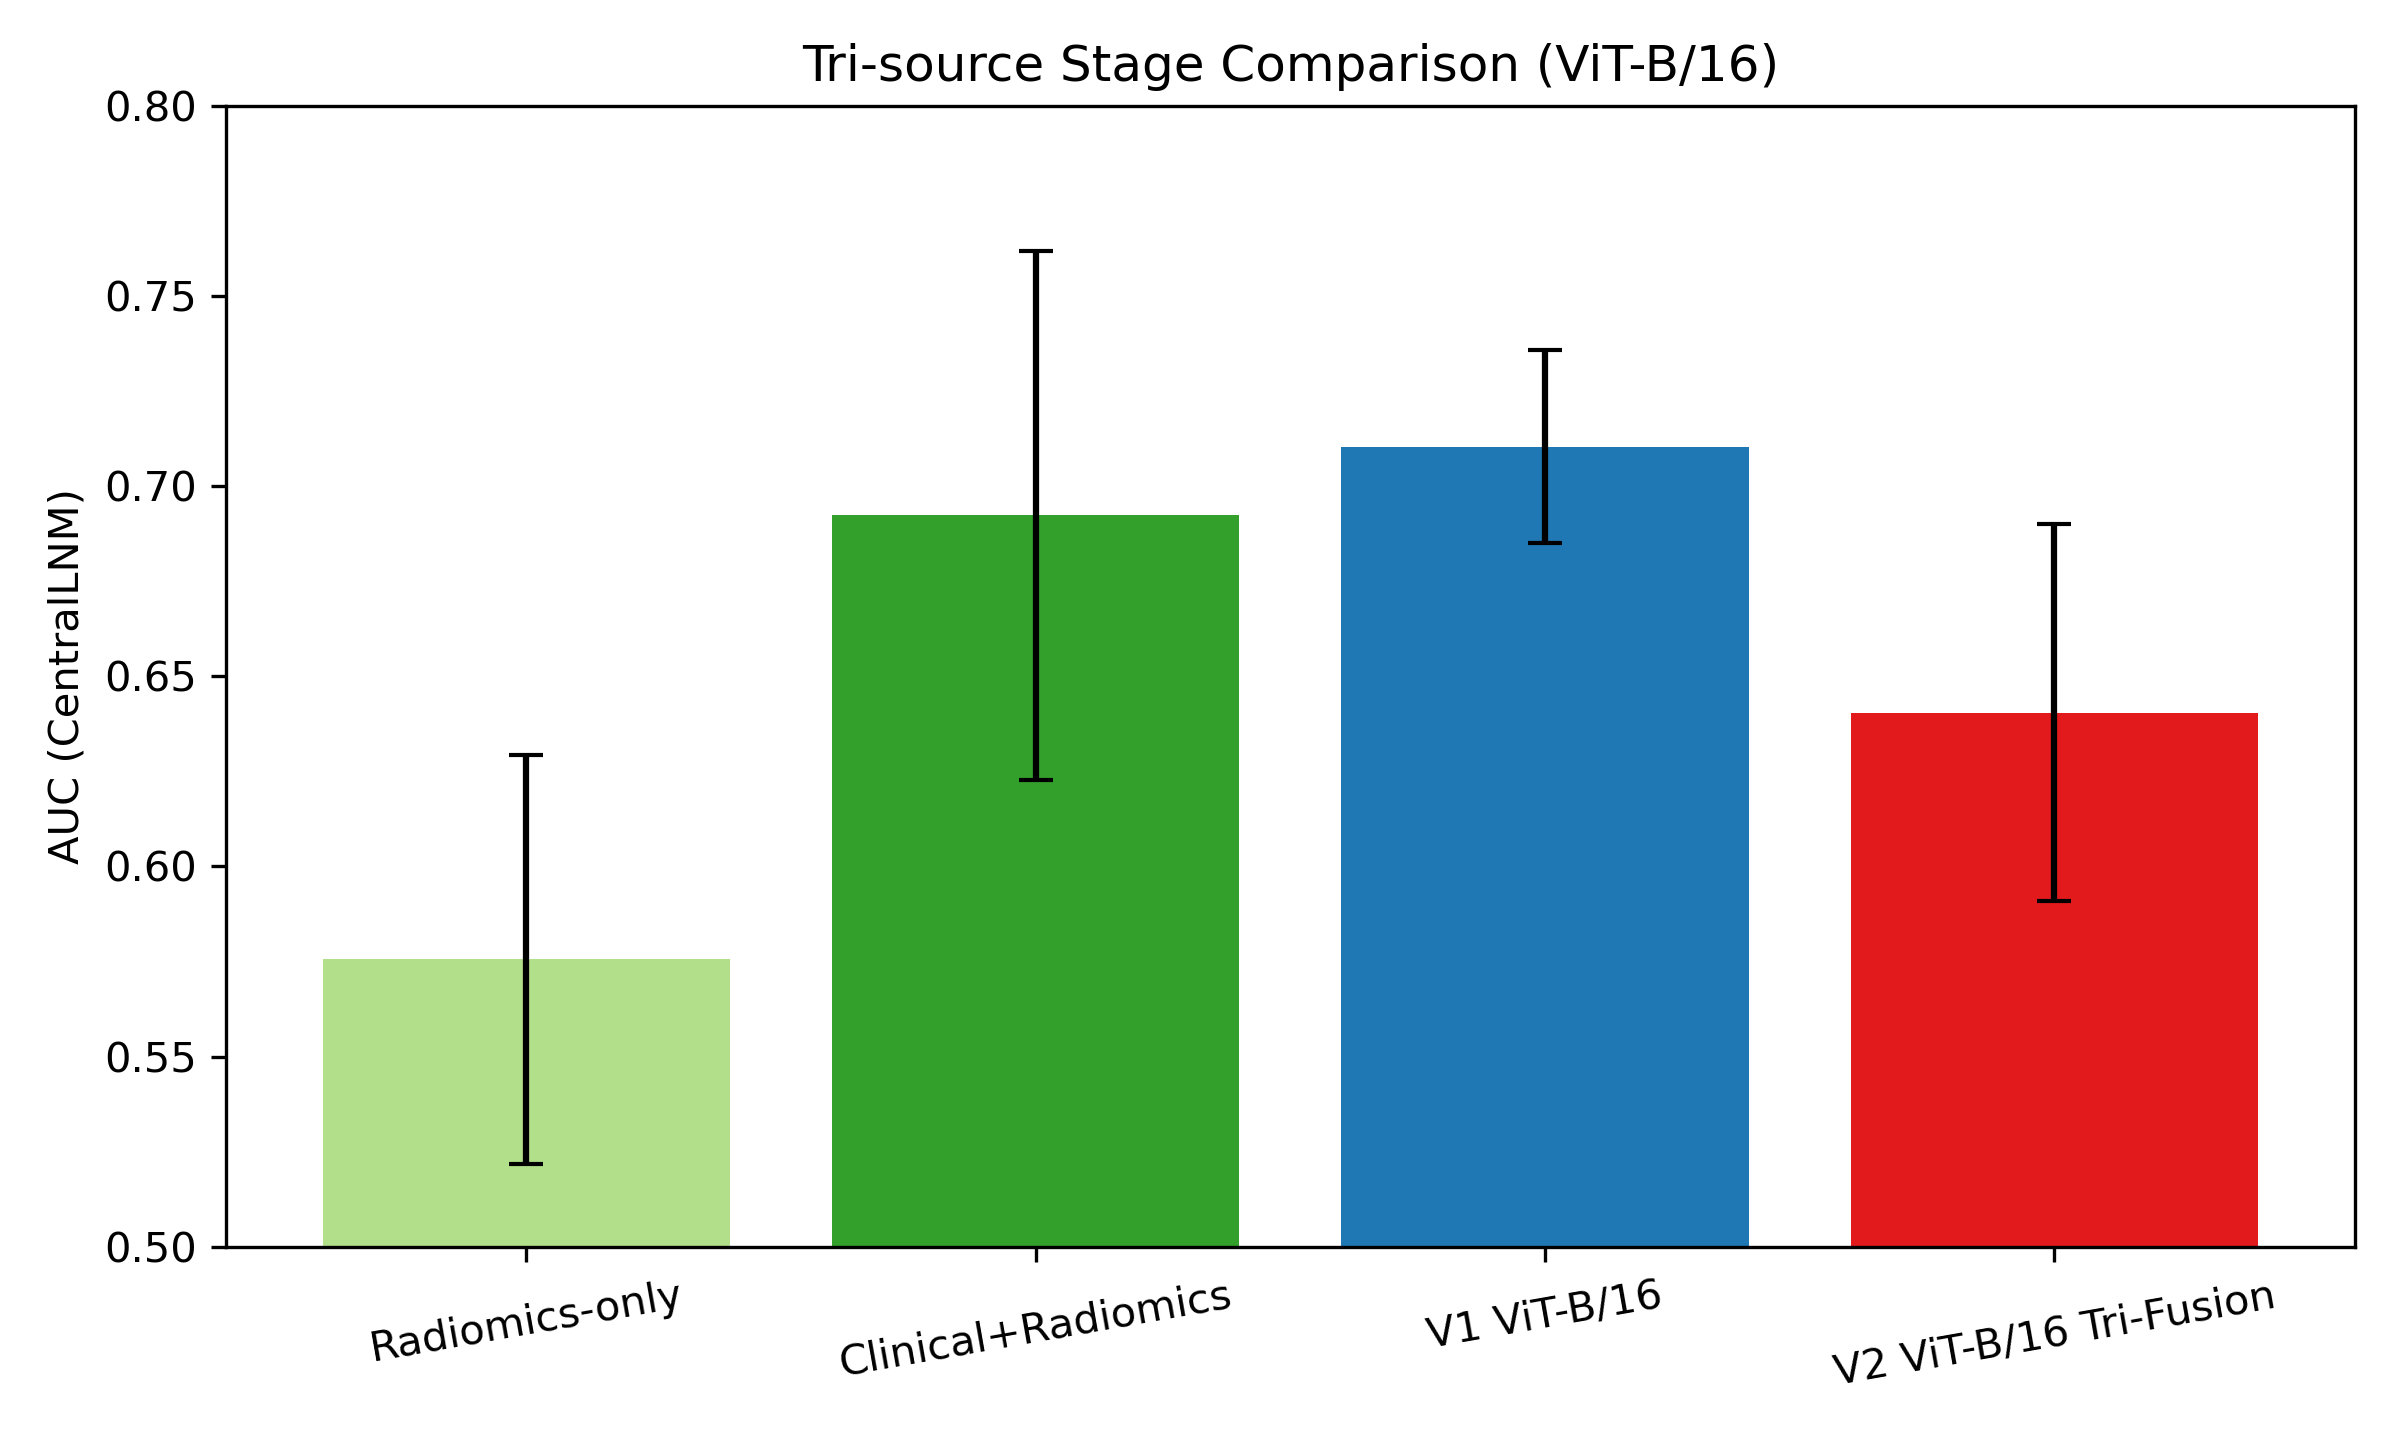
\includegraphics[width=0.82\textwidth]{figures/tri_source_auc_compare_vit_b16.png}
\caption{多源融合四组设置在 CentralLNM 任务上的 AUC 比较（ViT-B/16 版本）。}
\label{fig:tri_source_auc}
\end{figure}

\begin{figure}[H]
\centering
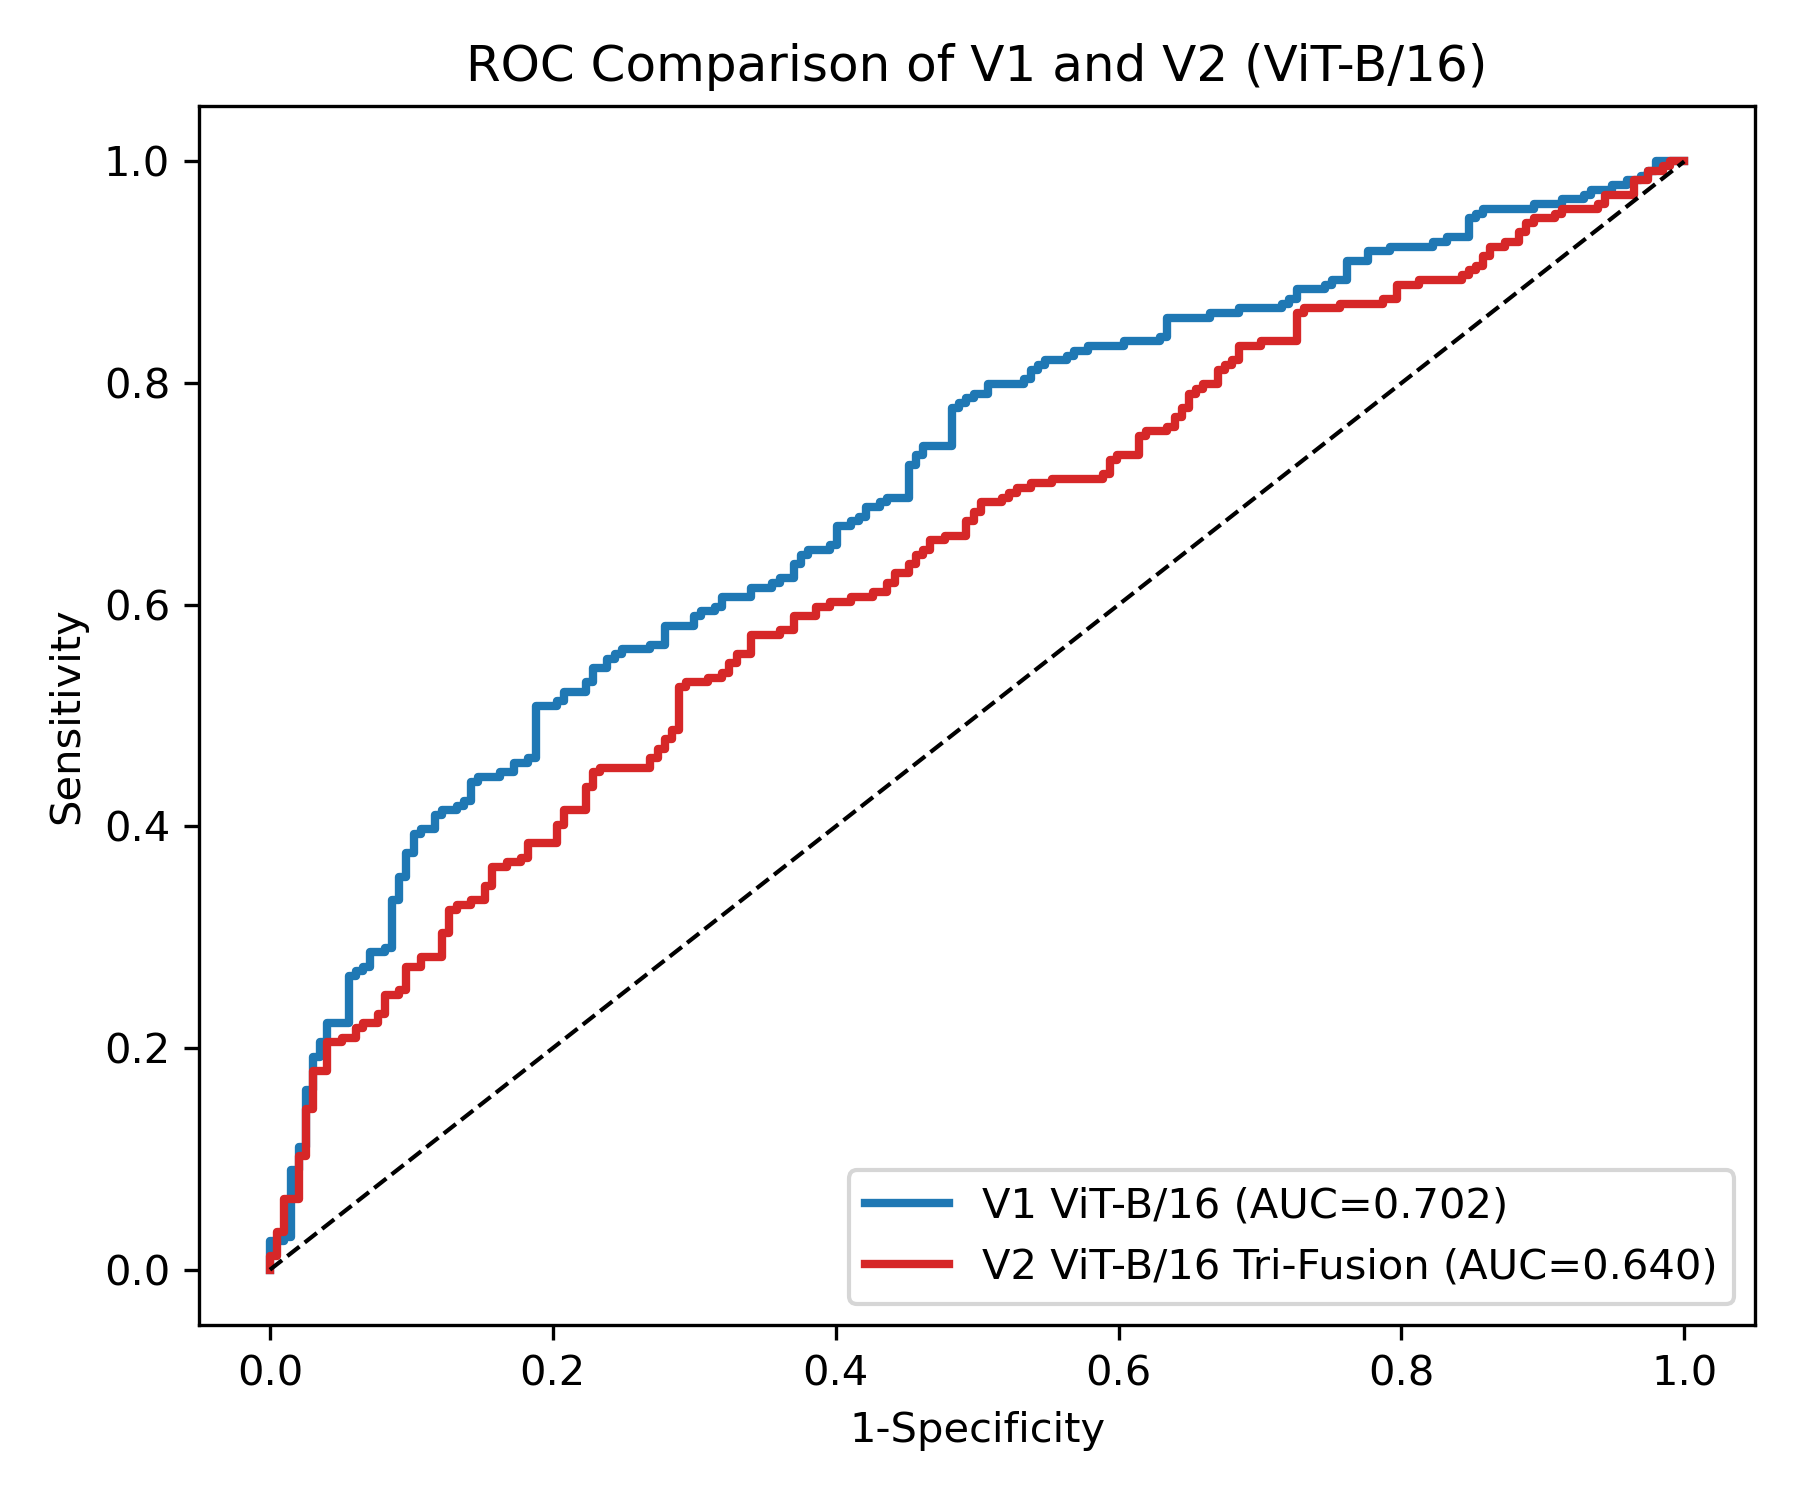
\includegraphics[width=0.82\textwidth]{figures/roi_radiomics_vs_tri_source_roc_vit_b16.png}
\caption{ViT-B/16 下 V1 与 V2 模型在 CentralLNM 任务上的 ROC 对比。}
\label{fig:tri_source_roc}
\end{figure}

其中，ViT-B/16 的 V1（Deep+Clinical）取得最高 AUC（0.7104$\pm$0.0253）；V2（Tri-Fusion）在当前配置下出现下降（0.6404$\pm$0.0496）。相对于原始临床基线，V1 仍保留正向增益，而 V2 已回落至基线以下。该结果提示，在高表征能力骨干下，组学分支的注入方式仍是性能瓶颈，而非“加入更多信息源即可自动增益”。
图~\ref{fig:tri_source_auc} 与图~\ref{fig:tri_source_roc} 共同显示，V2 相较 V1 的曲线整体下移，说明当前 ViT-B/16 版本的三源融合尚未形成稳定增益。该部分因此更适合作为方法学优化方向，而不是当前投稿主模型。

\subsection{代表性病例可视化分析}
为增强模型结果的临床可解释性，本研究补充展示了代表性病例的可视化证据。图~\ref{fig:case_slices_high} 展示高风险病例在多切面上的 Grad-CAM 响应，图~\ref{fig:case_modal_high} 展示同一病例在不同模态下的响应分布。

\begin{figure}[H]
\centering
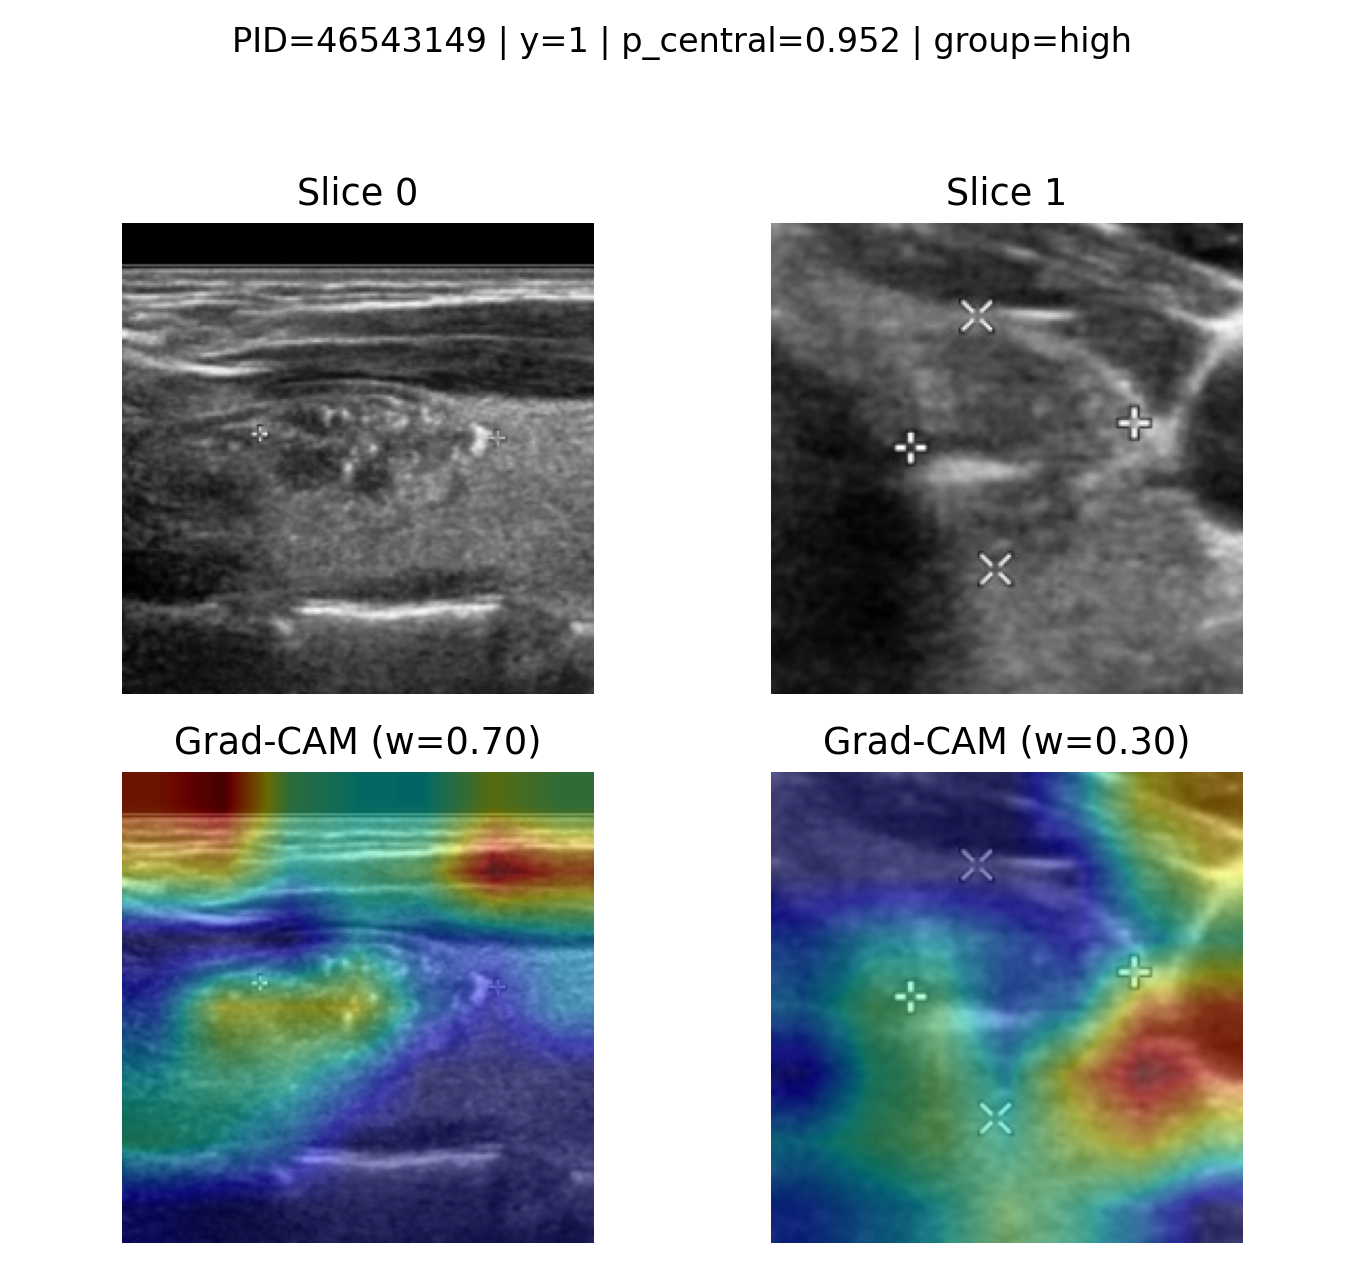
\includegraphics[width=0.92\textwidth]{figures/gradcam_slices_case_high.png}
\caption{高风险代表病例的多切面 Grad-CAM 可视化。模型在关键切面上呈现更集中激活，且与较高 CentralLNM 预测概率一致。}
\label{fig:case_slices_high}
\end{figure}

\begin{figure}[H]
\centering
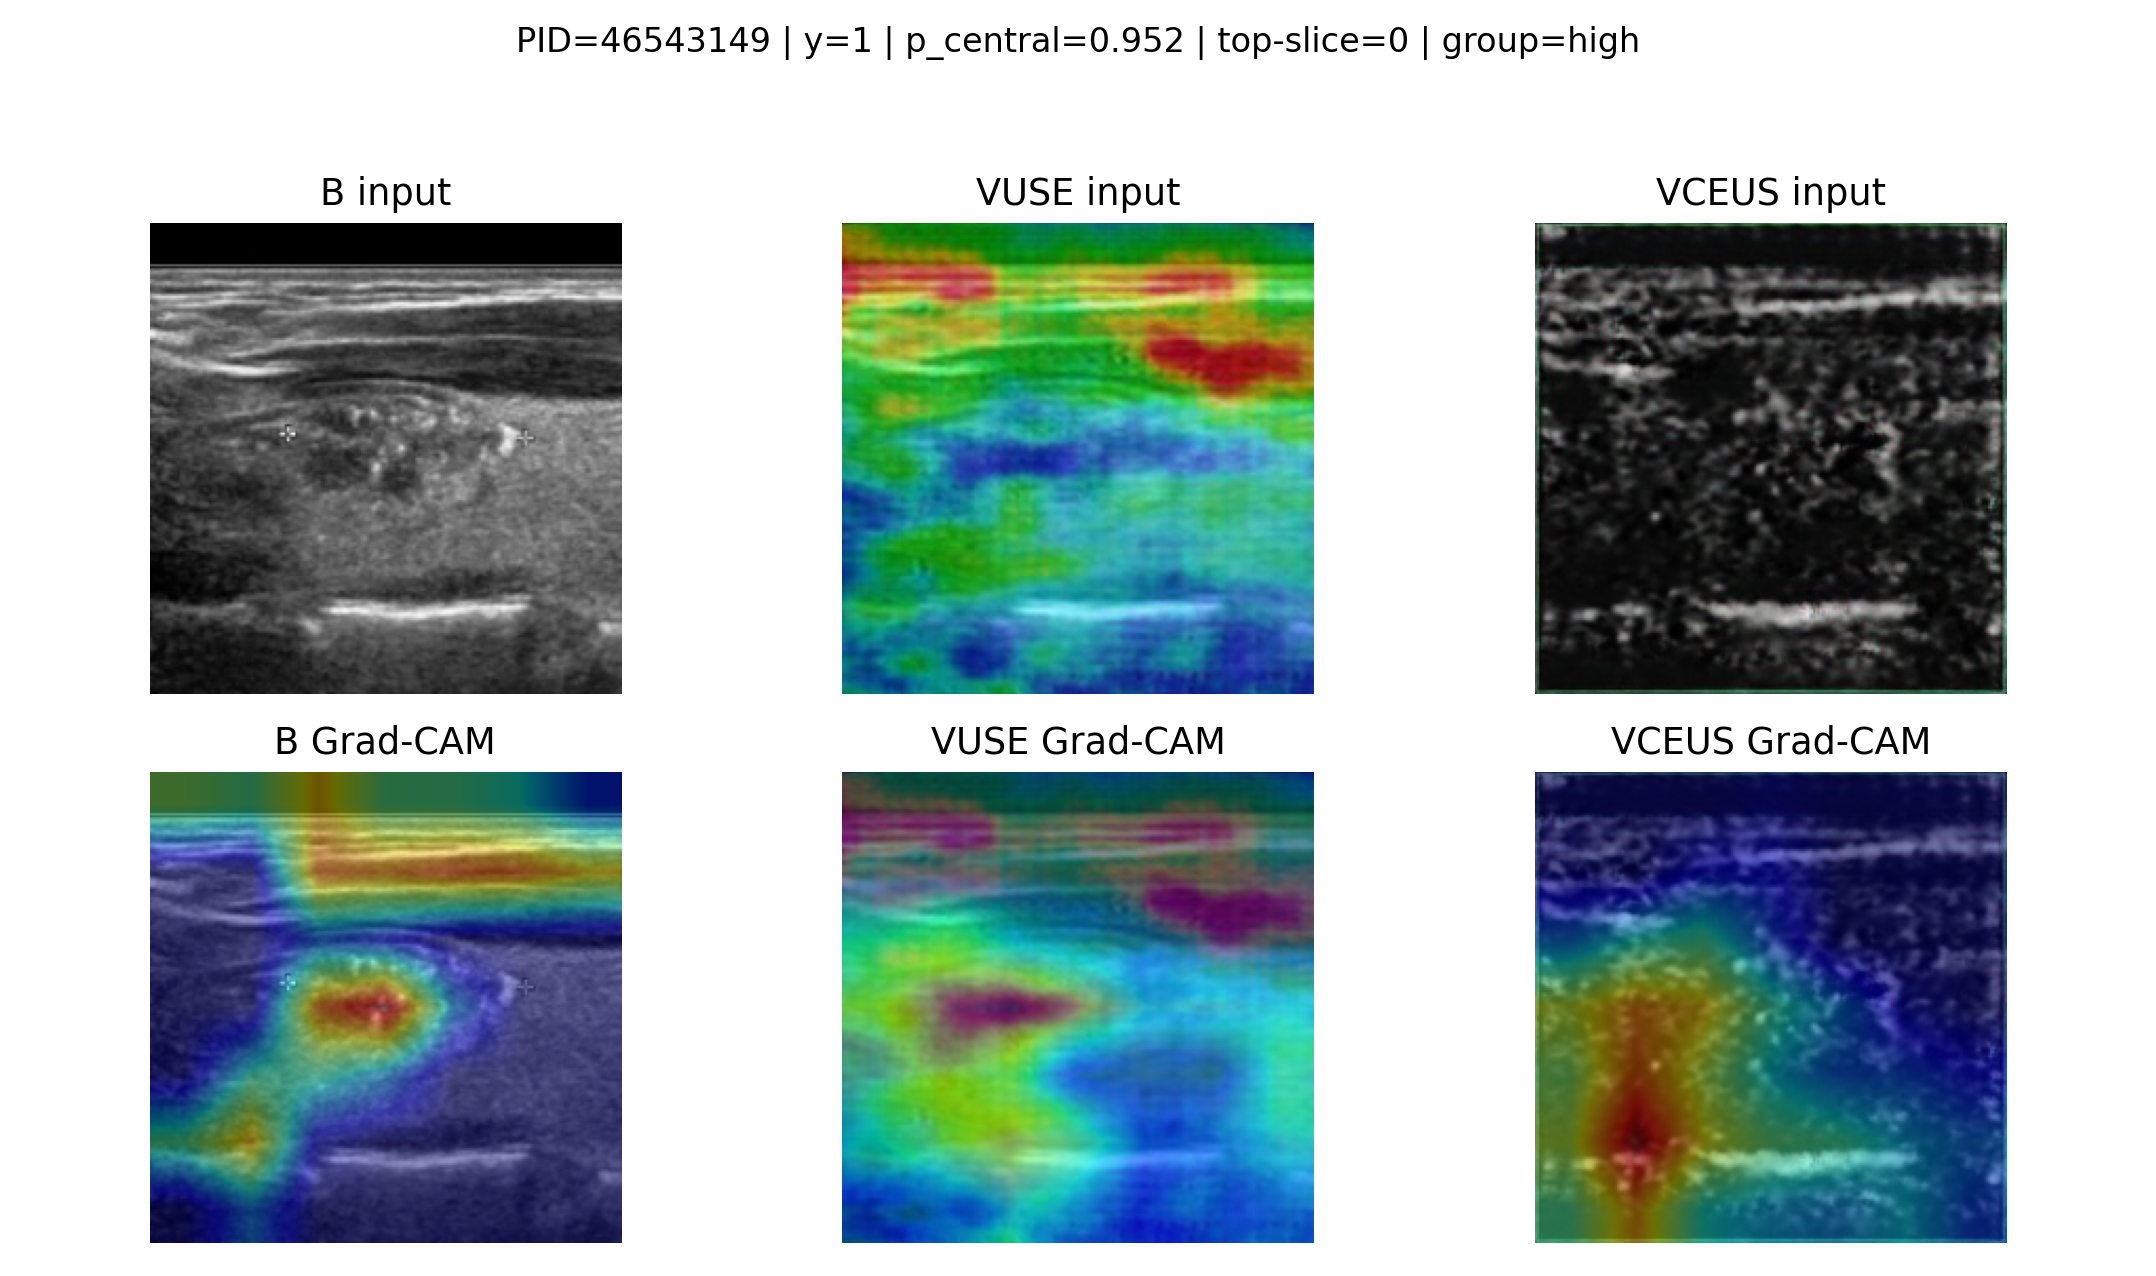
\includegraphics[width=0.92\textwidth]{figures/gradcam_modalities_case_high.png}
\caption{高风险代表病例的多模态 Grad-CAM 可视化。不同模态在关键区域呈现差异化响应，提示多模态信息具有互补性。}
\label{fig:case_modal_high}
\end{figure}

可视化结果提示，完整模型在高风险病例中的注意区域与临床关注区域具有较好一致性，同时模态间存在非冗余贡献。该证据与前述量化结果相互印证，即模型性能提升并非仅来自参数复杂度增加，而是来自患者级聚合与临床主导融合后对有效影像信息的更充分利用。为控制主文篇幅，其余中风险与低风险病例可视化结果置于补充材料。
